%%%%%%%%%%%%%%%%%%%%%%%%%%%%%% -*- Mode: Latex -*- %%%%%%%%%%%%%%%%%%%%%%%%%%%%
%% uhtest-appendix.tex -- 
%% Author          : Robert Brewer
%% Created On      : Fri Oct  2 16:31:12 1998
%% Last Modified By: Robert Brewer
%% Last Modified On: Mon Oct  5 14:41:05 1998
%% RCS: $Id: uhtest-appendix.tex,v 1.1 1998/10/06 02:07:03 rbrewer Exp $
%%%%%%%%%%%%%%%%%%%%%%%%%%%%%%%%%%%%%%%%%%%%%%%%%%%%%%%%%%%%%%%%%%%%%%%%%%%%%%%
%%   Copyright (C) 1998 Robert Brewer
%%%%%%%%%%%%%%%%%%%%%%%%%%%%%%%%%%%%%%%%%%%%%%%%%%%%%%%%%%%%%%%%%%%%%%%%%%%%%%%
%% 

\chapter{Baseline Assessment}
\label{baseline-assessment}
\begin{figure}[h]
\centering
\includegraphics[width=0.75\textwidth]{q1}
\caption{Baseline Assessment: Section 1.}
\end{figure}

\begin{figure}[h]
\centering
\includegraphics[width=0.75\textwidth]{q2}
\caption{Baseline Assessment: Section 2.}
\end{figure}

\begin{figure}[h]
\centering
\includegraphics[width=0.75\textwidth]{q3}
\caption{Baseline Assessment: Section 3.}
\end{figure}

\begin{figure}[h]
\centering
\includegraphics[width=0.75\textwidth]{q4}
\caption{Baseline Assessment: Section 3.}
\end{figure}

\begin{figure}[h]
\centering
\includegraphics[width=0.75\textwidth]{q5}
\caption{Baseline Assessment: Section 3.}
\end{figure}

\begin{figure}[h]
\centering
\includegraphics[width=0.75\textwidth]{q6}
\caption{Baseline Assessment: Section 4.}
\end{figure}

\begin{figure}[h]
\centering
\includegraphics[width=0.75\textwidth]{q7}
\caption{Baseline Assessment: Section 4.}
\end{figure}

\begin{figure}[h]
\centering
\includegraphics[width=0.75\textwidth]{q8}
\caption{Baseline Assessment: Section 5.}
\end{figure}

\chapter{RadGrad Data Model}
\label{data-model}
\subsection{Career Goals}
\begin{figure}[htbp!]
\centering
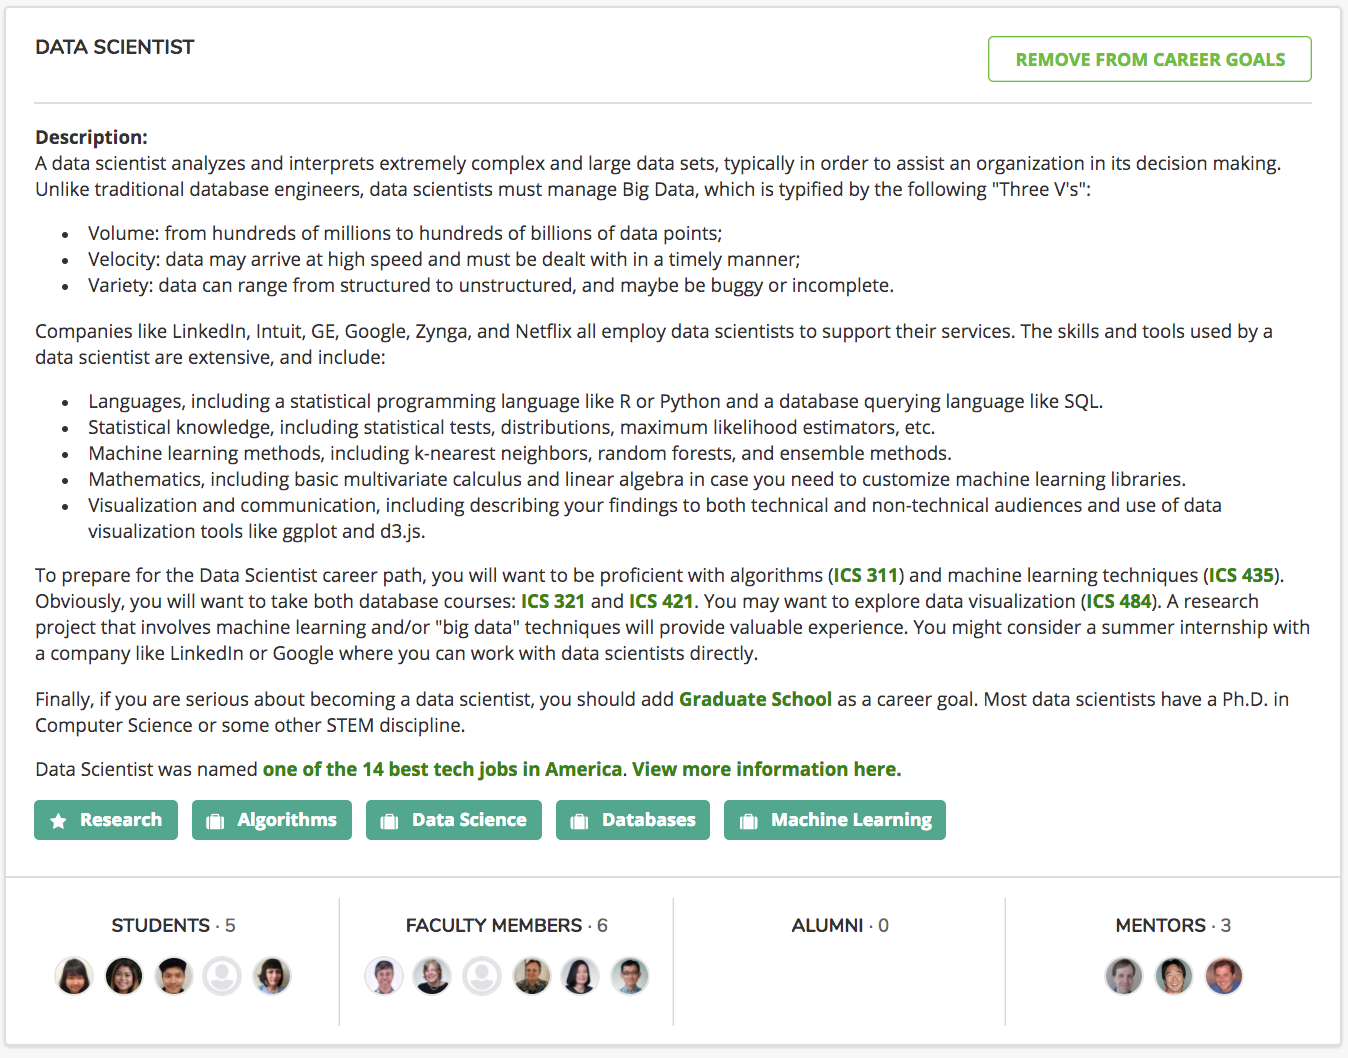
\includegraphics[width=1.0\textwidth]{dm-career}
\caption{Example of a career goal representation.}
\label{career-goal}
\end{figure}
Career goals represent possible ICS related careers that ICS students can aspire to get after graduation (Figure 6.1). Each career goal has an associated name, slug, description, related interests, and an optional URL for more information. Students can choose as many career goals as they want. Faculty and mentors can choose career goals that they would like to be associated with as well. Possible career goals as of June 2017 are listed in Table ~\ref{table:career-goals}.

\begin{table}[htbp!]
\centering
\begin{tabular}{ l l l } 
 Data Scientist & Database Administrator & DevOps Engineer \\ 
 Full Stack Developer & Game Developer & Graduate School \\ 
 Information Security Analyst & Information System Manager & IoT Architect \\ 
 Mobile App Developer & Network Engineer & Research Scientist \\
 Robotics Engineer & Software Developer & Startup Co-Founder \\
 Teacher & UX Designer & VR/AR Engineer 
\end{tabular}
\caption{List of RadGrad career goals as of June 2017}
\label{table:career-goals}
\end{table}

\subsection{Courses}
\begin{figure}[htbp!]
\centering
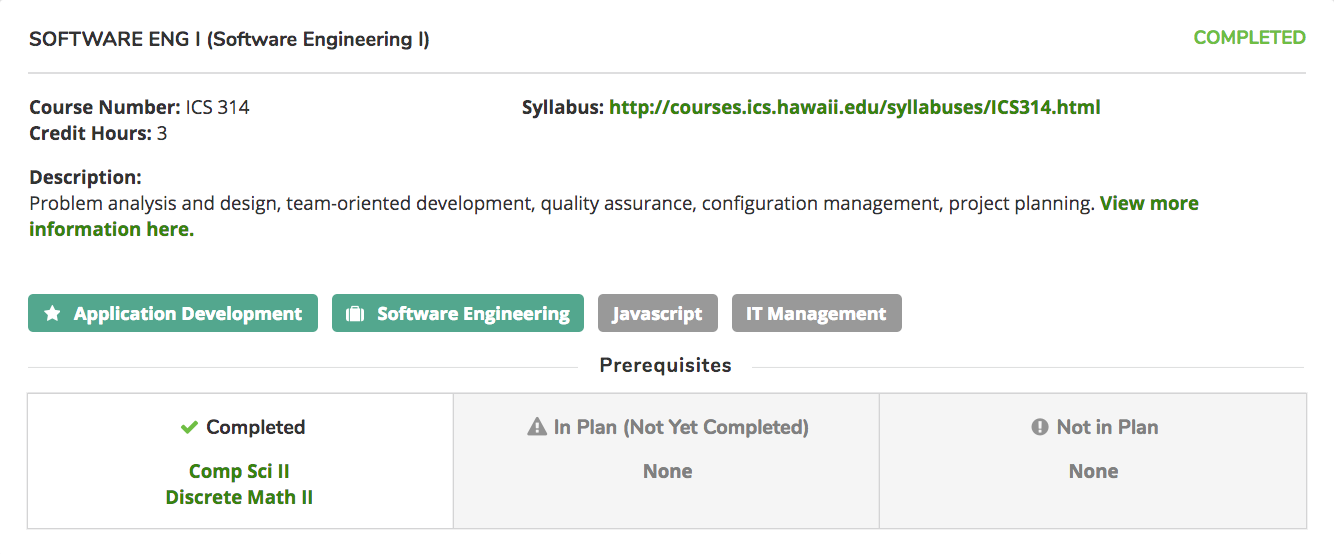
\includegraphics[width=1.0\textwidth]{dm-course}
\caption{Example of a course representation.}
\label{course}
\end{figure}
Courses represent all past, present, and future ICS courses (Figure ~\ref{course}). Each course has an associated name, short name, slug, course number, description, credit hours, related interests, a syllabus URL, a URL for more information, and associated prerequisites. The course name is the official name appearing in the UH registration guide, and the course short name is used for display purposes. Students may add as many courses as they would like to their degree plan. 

Course instances represent individual instances for each student. Each course instance has an associated semester, course, whether it has been verified or not, whether it came from STAR or not, grade, credit hours, note, student, and associated ICE points. A past course instance is always considered verified if it is from STAR. Course instances from STAR from the current or future semesters are not considered verified yet since there is no official grade. Special courses that are manually input (not from STAR) could also be considered verified by an advisor. A course instance has a note if it is not an ICS course. It is important to note that course instances on RadGrad are only valid on RadGrad, and students must use other methods to officially make UH course registration changes.

\subsection{Desired Degrees}
\begin{figure}[htbp!]
\centering
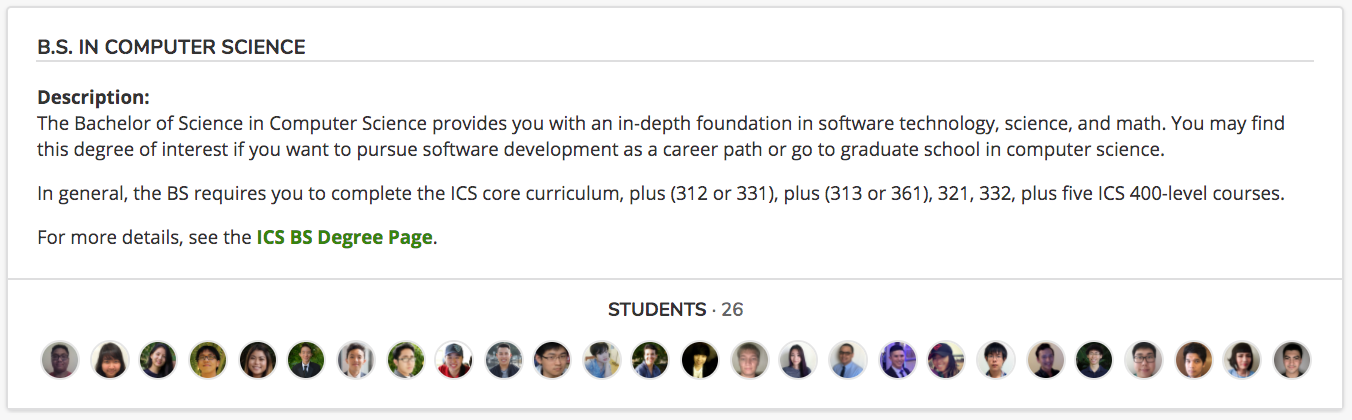
\includegraphics[width=1.0\textwidth]{dm-degree}
\caption{Example of a desired degree representation.}
\label{desired-degree}
\end{figure}
Desired degrees represent all past, present, and future ICS degrees (Figure ~\ref{desired-degree}). Each desired degree has an associated name, short name, slug, and description. Students can only choose one desired degree at any given time. However, they are free to switch desired degrees as many times as they want. It is important to note that desired degrees on RadGrad are only valid on RadGrad, and students must use other methods to officially change their declared degree at UH. 

\subsection{Degree Plan}
\begin{figure}[htbp!]
\centering
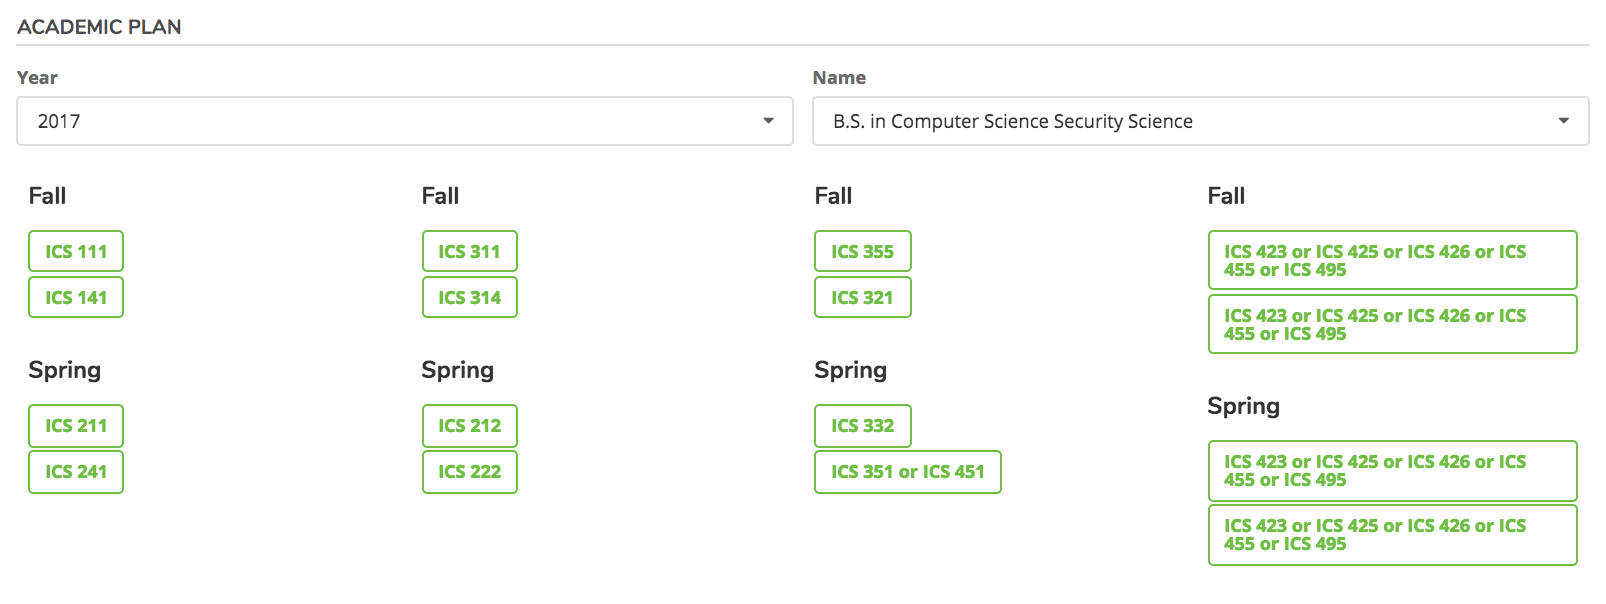
\includegraphics[width=1.0\textwidth]{dm-degreeplan}
\caption{Example of a degree plan representation.}
\label{degree-plan}
\end{figure}
Degrees plans represent all past, present, and future ICS degree plans (Figure ~\ref{degree-plan}). Each degree plan has an associated degree, name, effective semester, amount of courses per semester, and list of courses. Students can view degree plans if they would like a more specific focus than just a broad BS or BA degree. Examples of degree plans are ``BS in Computer Sciences Security Sciences", ``BA in ICS Security Science Focus", and ``BA in Computer Sciences IT Focus." Students can look at any plan at any time to see what they would need to do to fulfill it. It is important to note that these degree plans change over time, and a ``BS in Computer Sciences Security Sciences" may be different in 2016 than in 2018. This is why both year and plan name must be chosen when selecting a plan.  Degree plans were created to help students to become more aware of and make sense of the different degree plans that they can choose from. Having these representations on RadGrad help students to see how different degree plans would work with their specific interests, career goals, courses, and opportunities. Overall, degree plans can help students to narrow down their interests into a more specific field. 

\subsection{Feeds}
\begin{figure}[htbp!]
\centering

\includegraphics[width=0.5\textwidth]{dm-feed}
\caption{Example of a feed representation.}
\label{feed}
\end{figure}
Feeds represent select actions of RadGrad users (Figure ~\ref{feed}). Each feed has associated users, opportunity, course, semester, description, time stamp of the action, picture, and feed type. A feed could have one or multiple users. There are currently six different feed types: a new RadGrad user is added, a new course is added to RadGrad, a new opportunity is added to RadGrad, a user has been verified for completing an opportunity, a new course review has been added, and a new opportunity review has been added. These particular actions have been selected because they could be useful and of interest to other RadGrad users.

\subsection{Feedbacks}
\begin{figure}[htbp!]
\centering
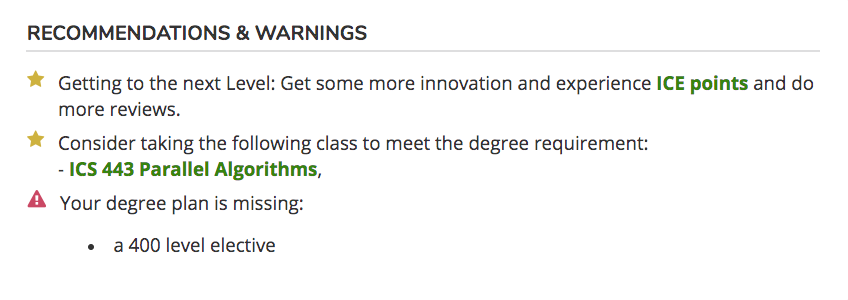
\includegraphics[width=1.0\textwidth]{dm-feedback}
\caption{Example of feedback representations.}
\label{feedback}
\end{figure}
Feedbacks represent recommendations and warnings for students (Figure ~\ref{feedback}). Each feedback has an associated name, slug, description, and feedback type. There are currently two feedback types: recommendation and warning. 

Feedback instances represent individual instances for each student. Each feedback instance has an associated feedback, user, description, and area. There are currently four different areas: interests, ICE, STAR, and degree plan. Each time the student's plan changes, feedback instances in these areas are deleted and recalculated.

\subsection{Help Messages}
\begin{figure}[htbp!]
\centering
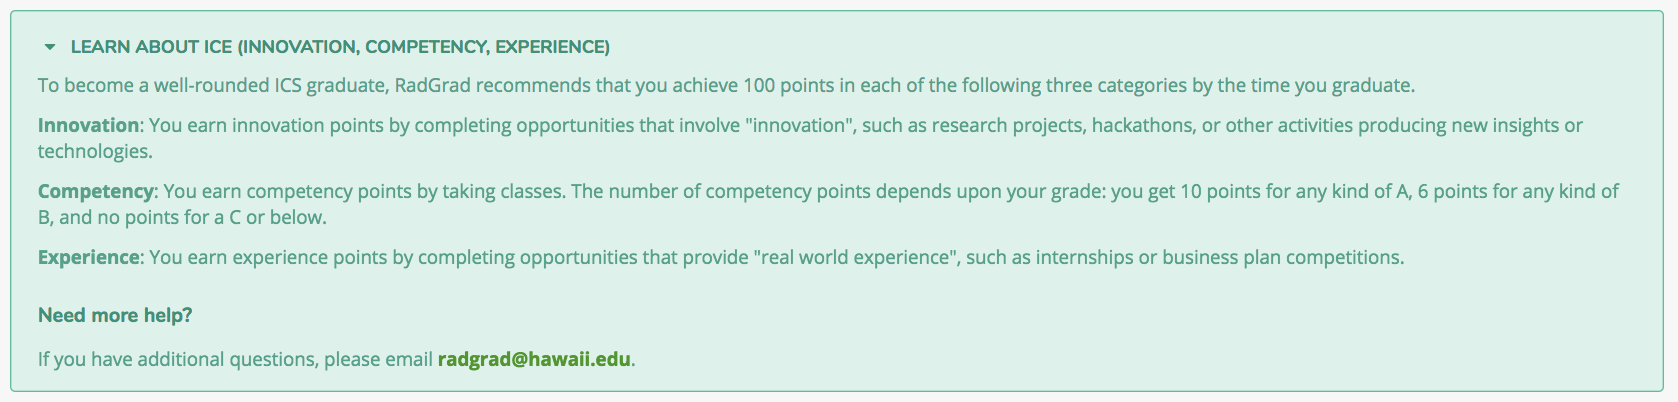
\includegraphics[width=1.0\textwidth]{dm-help}
\caption{Example of a help representation.}
\label{help}
\end{figure}
Help messages represent guidance for a particular RadGrad page (Figure ~\ref{help}). Each help message has an associated route name, title, and text. The text can contain actual text, images, and formatting. Each page (route name) can have at most one help message. These help messages are displayed at the top of the specified page, in a collapsible pane.  

\subsection{ICE}
\begin{figure}[htbp!]
\centering
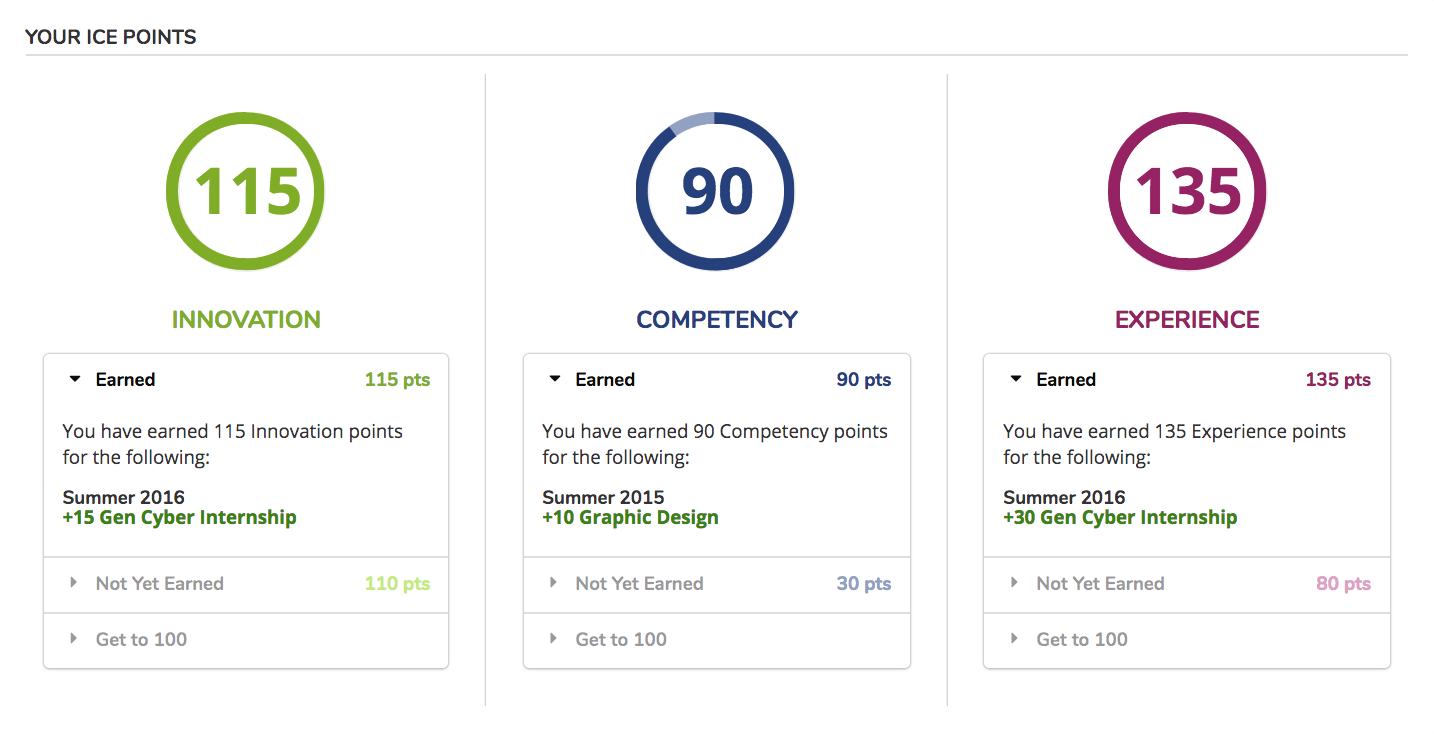
\includegraphics[width=1.0\textwidth]{dm-ice}
\caption{Example of an ICE representation.}
\label{ice}
\end{figure}
ICE represents a student's ICE points (Figure ~\ref{ice}). Each ICE has an associated number for ``I", ``C", and ``E." There are two types of ICE points: earned and planned. Earned ``I" and ``E" points are calculated by adding the ``I" or ``E" points for each verified opportunity in the student's plan. Earned ``C" points are calculated by adding the ``C" points for each verified course in the student's plan. The amount of earned points for each course depends on the grade that the student received; A's represent more points than B's. Planned ``I" and ``E" points are calculated by adding the ``I" or ``E" points for each unverified opportunity in the student's plan. Planned ``C" points are calculated by adding the ``C" points for each unverified course in the student's plan. A student's earned and planned ICE points are updated each time there are changes to the student's degree plan. 

\subsection{Interests}
\begin{figure}[htbp!]
\centering
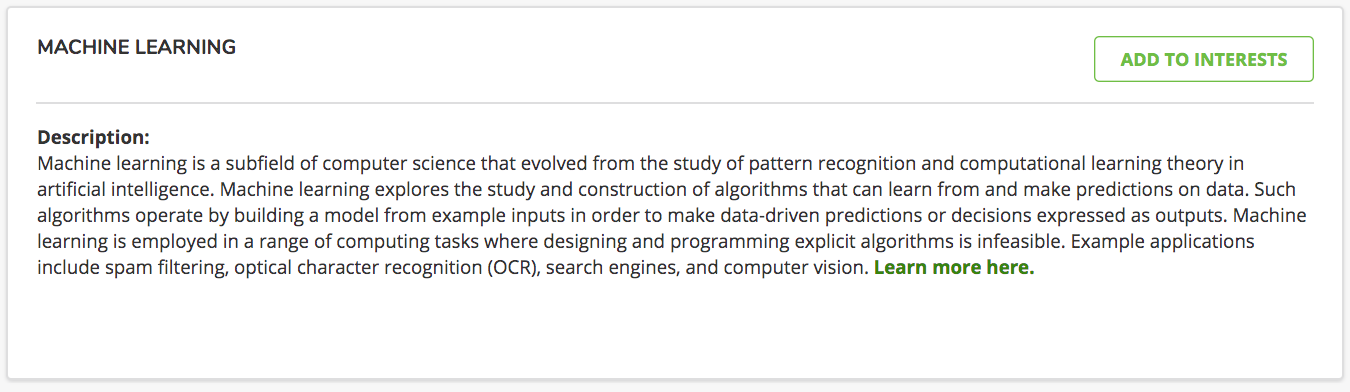
\includegraphics[width=1.0\textwidth]{dm-interests}
\caption{Example of an interest representation.}
\label{interests}
\end{figure}
Interests represent possible ICS related interests that RadGrad users could have (Figure ~\ref{interests}). Each interest has an associated name, slug, description, interest type, and a URL for more information. All RadGrad users may choose to be associated with as many interests as they would like. All current interests on RadGrad as of June 2017 are listed in Table ~\ref{table:interests}.

\begin{table}[htbp!]
\centering
\begin{tabular}{ l l l } 
.NET & Algorithms & Android \\ 
Application Development & Artificial Intelligence & Assembler \\
Bioinformatics & Biology & C and C++ \\
C\# & Civic Engagement & Cognitive Science \\
Computer Architecture & Computer Ethics & Computer Graphics \\
Computer Vision & Cryptography & Data Science \\
Data Visualization & Databases & Entrepreneurship \\
Game Design & Graphic Design & Hardware \\
High Performance Computing & Human-Computer Interaction & IT Management \\
Java & Javascript & Linux \\
Lisp & Machine Learning & Mobile Computing \\
Networks & Operating Systems & Parallel Programming \\
Perl & Prolog & Psychology \\
Python & R & Research \\
Robotics & Ruby & Software Development \\
SQL & Security & Sustainability \\
Teaching & Theory of Computation & Unity \\
Virtual Reality & Web Development & iOS
\end{tabular}
\caption{List of RadGrad interests as of June 2017}
\label{table:interests}
\end{table}

\subsection{Levels}
\begin{figure}[htbp!]
\centering
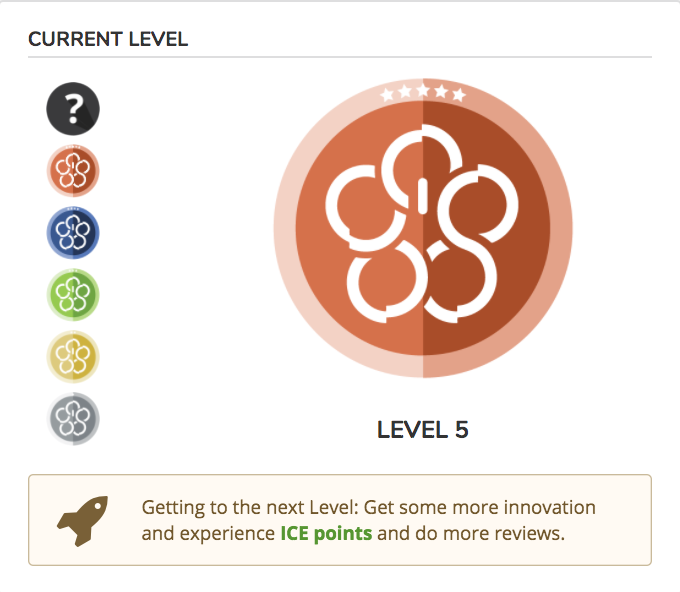
\includegraphics[width=0.5\textwidth]{dm-level}
\caption{Example of a level representation.}
\label{levels}
\end{figure}
Levels represent a student's RadGrad level (Figure ~\ref{levels}). There are six possible levels, from Level 1 to Level 6. A student's level is calculated based off the amount of ICS courses they have passed, the amount of opportunities they have done, and the amount of reviews they have contributed on RadGrad. Levels can be recalculated for all users at any time through the administrator pages.

\subsection{Advisor Logs}
\begin{figure}[htbp!]
\centering

\includegraphics[width=1.0\textwidth]{dm-log}
\caption{Example of an advisor log representation.}
\label{log}
\end{figure}
Advisor logs represent an interaction between an ICS advisor and a student (Figure ~\ref{log}). Each advisor log has an associated student, advisor, text, and date created. A new log can be created by the advisor whenever they have a meeting with a student. Advisors and students can use these logs to keep track of when meetings were held, and what occurred at these meetings. 

\subsection{Mentors}
\begin{figure}[htbp!]
\centering

\includegraphics[width=0.5\textwidth]{dm-mentor}
\caption{Example of a mentor representation.}
\label{mentor}
\end{figure}
The mentor data model includes three parts: mentor profiles, mentor questions, and mentor answers (Figure ~\ref{mentor}). Each mentor profile has an associated mentor, company, career, location, LinkedIn, and a message about what motivated them to become a mentor. Each mentor will have exactly one mentor profile.  

Each mentor question has an associated title, slug, student, whether it is moderated or not, whether it is visible or not, and moderator comments. Students can create as many mentor questions as they would like. However, each question needs to be approved by moderation in order to be visible to the public. Advisors and administrators have the ability to moderate questions. If a question is declined by moderation, the moderator can add reasons for the decline in the moderator comments field. The student can then see the feedback, and they are able to either edit their question and send it back to moderation, or simply discard the question. There is no limit to how long the back and forth process between student and moderator can go on. 

Each mentor answer has an associated question, mentor, and text. Each mentor question can have any amount of mentor answers, but each mentor answer can answer at most one mentor question. Each mentor question can only be associated with exactly one mentor. There is no moderation process for mentor answers, and submitted mentor answers are automatically visible on RadGrad. 

\subsection{Opportunities}
\begin{figure}[htbp!]
\centering
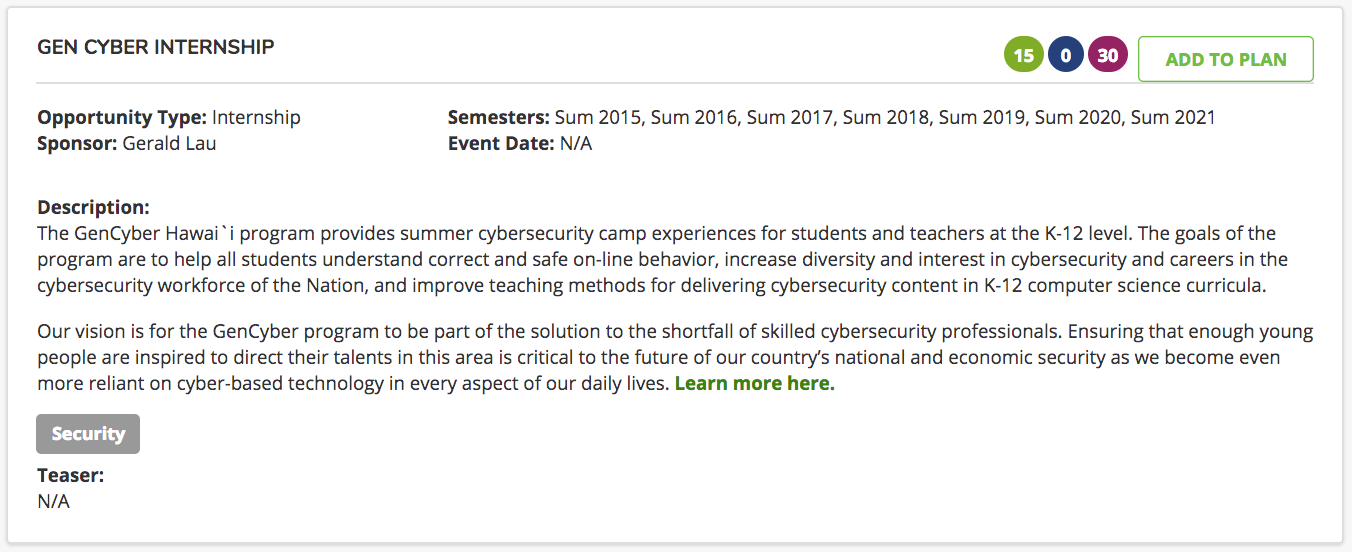
\includegraphics[width=1.0\textwidth]{dm-opportunity}
\caption{Example of an opportunity representation.}
\label{opportunity}
\end{figure}
Opportunities represent all past, present, and future ICS related opportunities (Figure ~\ref{opportunity}).  Each opportunity has an associated name, slug, description, opportunity type, sponsor, related interests, icon, semesters available, event date, whether it is an independent study or not, URL for more information, and ICE points. Currently, there are five opportunity types: club, event, internship, online learning, and project. The opportunity sponsor is any faculty member who is the point of contact for the opportunity. If the opportunity occurs on a semester basis, it will have associated semesters. If the opportunity occurs on a specific date, it will have an associated event date. The amount of ICE points varies depending on the nature of the opportunity, and is determined by RadGrad administrators. 

Opportunity instances represent individual instances for each student. Each opportunity instance has an associated semester, opportunity, whether it is verified or not, student, and ICE points. An opportunity instance can only be verified by a RadGrad advisor or faculty. Two students that each have an opportunity instance for the same opportunity could have different ICE points depending on the extent of their involvement in the opportunity.    

\subsection{Public Stats}
\begin{figure}[htbp!]
\centering
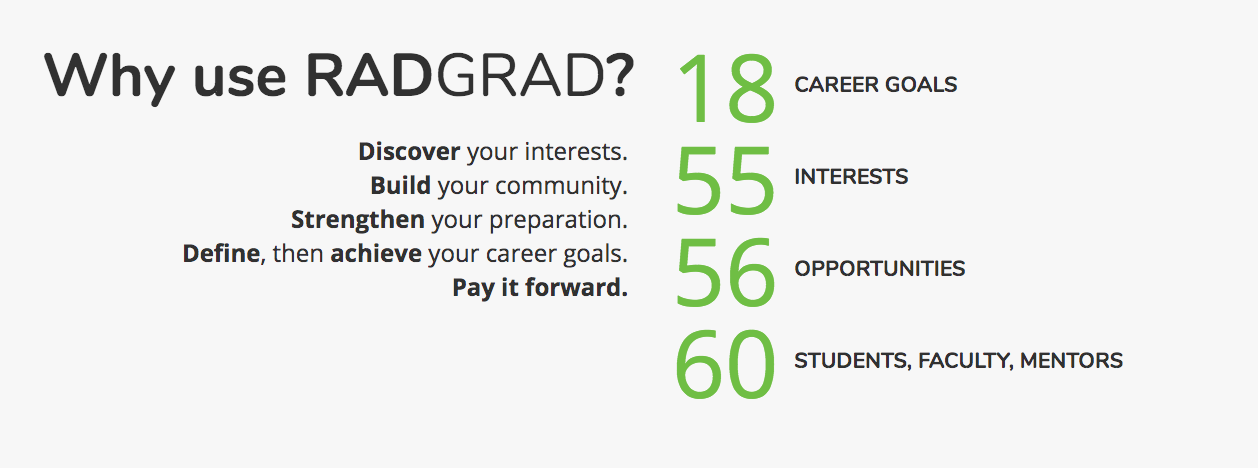
\includegraphics[width=1.0\textwidth]{dm-stats}
\caption{Example of a public stats usage on the landing page.}
\label{public-stats}
\end{figure}
Public stats calculate 24 different RadGrad statistics from the current database (Figure ~\ref{public-stats}). The statistics calculated are: total courses, total career goals, list of career goals, total desired degrees, list of desired degrees, total interests, list of interests, total opportunities, total project opportunities, list of project opportunities, total users, total students, total faculty, total mentors, list of mentor professions, list of mentor locations, total course reviews, list of courses reviewed, total level one students, total level two students, total level three students, total level four students, total level five students, and total level six students. Public stats are automatically recalculated once each day at midnight. 

\subsection{Reviews}
\begin{figure}[htbp!]
\centering
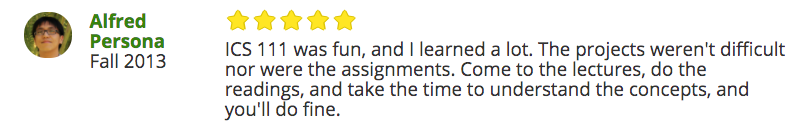
\includegraphics[width=1.0\textwidth]{dm-review}
\caption{Example of a review representation.}
\label{review}
\end{figure}
Reviews represent all course and opportunity reviews written by students on RadGrad (Figure ~\ref{review}). Each review has an associated slug, student, review type, reviewee, semester, rating, comments, whether it is moderated or not, whether it is visible or not, and moderator comments. There are two review types: course and opportunity. The reviewee refers to the course or opportunity that is being reviewed. Each review must have a rating from one to five stars (Figure ~\ref{ratings}). Each student may review a course once the semester they have taken it in has passed. Each student may review an opportunity once the opportunity has been verified. Each student can review each course or opportunity at most once. Each review is visible to the public by default, but can be removed by moderators. Advisors and administrators have the ability to moderate reviews. If a review is declined by moderation, the moderator can add reasons for the decline in the moderator comments field. The student can then see the feedback, and they are able to either edit their review and send it back to moderation, or simply discard the review. There is no limit to how long the back and forth process between student and moderator can go on. A student can also update their review at any time, but this will mean that the review will go through the moderation process again.

\begin{figure}[htbp!]
\centering
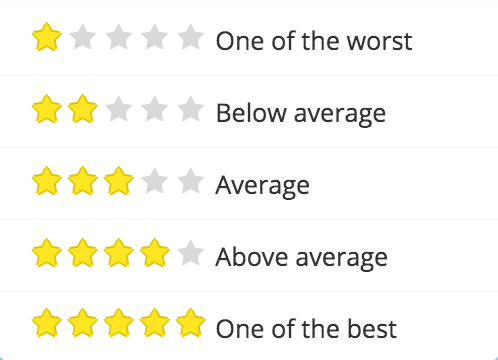
\includegraphics[width=0.3\textwidth]{datamodel-reviews}
\caption{Course and opportunity review ratings.}
\label{ratings}
\end{figure}

\subsection{Roles}
Roles represent the different user roles allowed in RadGrad. There are currently six roles: faculty, student, admin, alumni, advisor, and mentor. Currently, users are allowed to have exactly one role. All users except for admin and advisor can view only their own RadGrad pages. Advisors can also view student RadGrad pages, and admin can view all RadGrad pages. 

\subsection{Semesters}
Semesters represent an academic semester at the University of Hawaii. Each semester has an associated term, year, number to sort by, semester number, and slug. There are three possible terms: Spring, Summer, and Fall. The number to sort by easily allows chronological comparisons between semesters. Semester number is another number used for sorting semesters, using 2010 as the earliest year. 

\subsection{Slugs}
Slugs are strings used as part of a URL to uniquely identify an entity. These strings do not change with different instantiations of the database like docIDs do. Slugs are used in the RadGrad data model to represent relationships between different entities. Therefore, only collections that need to be referenced by other collections contain a slug. 

\subsection{Teasers}
\begin{figure}[htbp!]
\centering
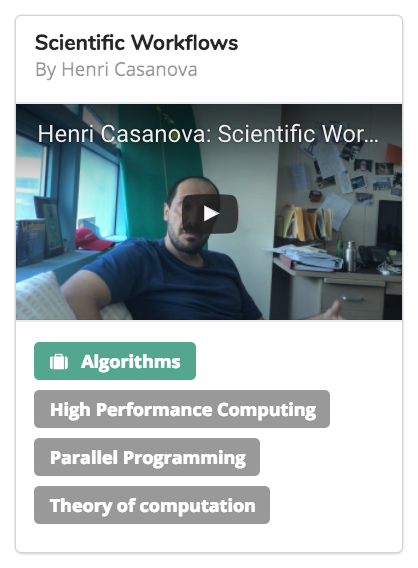
\includegraphics[width=0.5\textwidth]{dm-teaser}
\caption{Example of a teaser representation.}
\label{teaser}
\end{figure}
Teasers represent short videos that advertise an ICS opportunity (Figure ~\ref{teaser}). Each teaser has an associated title, slug, author, URL, description, duration, related interests, and opportunity. Any member of RadGrad can be an author of a teaser. Teasers are typically less than a minute long and function as a sort of quick advertisement to get potential students interested in participating in that particular opportunity. 

\subsection{Users}
\begin{figure}[htbp!]
\centering
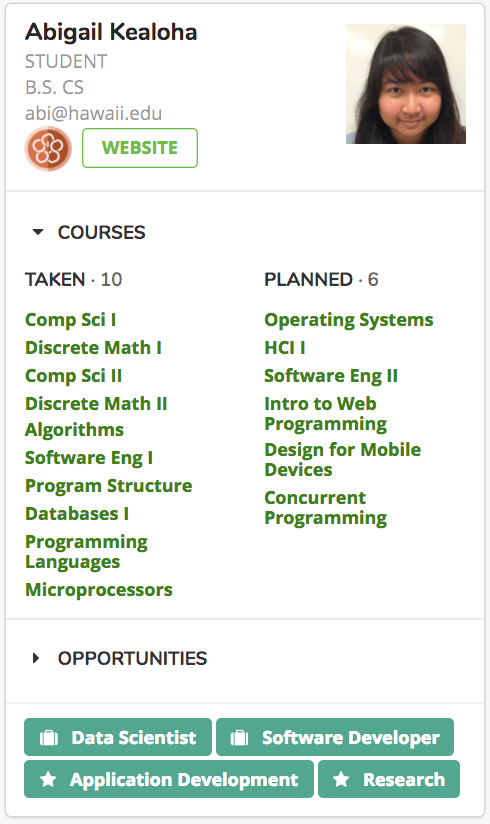
\includegraphics[width=0.5\textwidth]{dm-user}
\caption{Example of user representations.}
\label{user}
\end{figure}
Users represent anyone who has created an account on the RadGrad system (Figure ~\ref{user}). Each user has an associated username, first name, last name, slug, email, password, UH ID, career goals, interests, desired degree, picture, level, website, hidden courses, and hidden opportunities. The user's RadGrad username is the same as their UH email name. This, along with their email, cannot be changed once the user's account is created. Only student users will have a desired degree and a level. Hidden courses and hidden opportunities are used to keep track of courses and opportunities that students have actively ``hidden" from their page. By keeping track of these hidden courses and opportunities, students can have the option to make them visible again.

\subsection{Verification Requests}
\begin{figure}[htbp!]
\centering

\includegraphics[width=1.0\textwidth]{dm-verification}
\caption{Example of a verification request representation.}
\label{verification-request}
\end{figure}
Verification requests represent a request from a student to get verification and ICE points for completing an opportunity (Figure ~\ref{verification-request}). Each opportunity has an associated date, status, verifier, and feedback. There are three possible statuses: accepted, rejected, and open. The verifier is the user who has verified the event. Only advisors, faculty, and admin can be a verifier. If a request is rejected, the verifier can add reasons for the rejection in the feedback field. The student can then see the feedback and the results of the verification. If the verifier wishes to reopen the verification request, they may do so at any time. A student who would like to reopen a request will need to contact the verifier.  

\subsection{Academic Years}
Academic years represent an academic year at the University of Hawaii. Each academic year has an associated year, spring year, student, and semesters. Since academic years start in the Fall and end in the Summer, they span two years: year, and spring year. A student on RadGrad must have an academic year for each year, or portion of a year, that they are enrolled in an ICS course or participated in an ICS opportunity.

\chapter{Other RadGrad User Components}
\label{other-radgrad-components}
\section{Advisor Mode}
\subsection{Student Configuration}
\begin{figure}[htbp!]
\centering
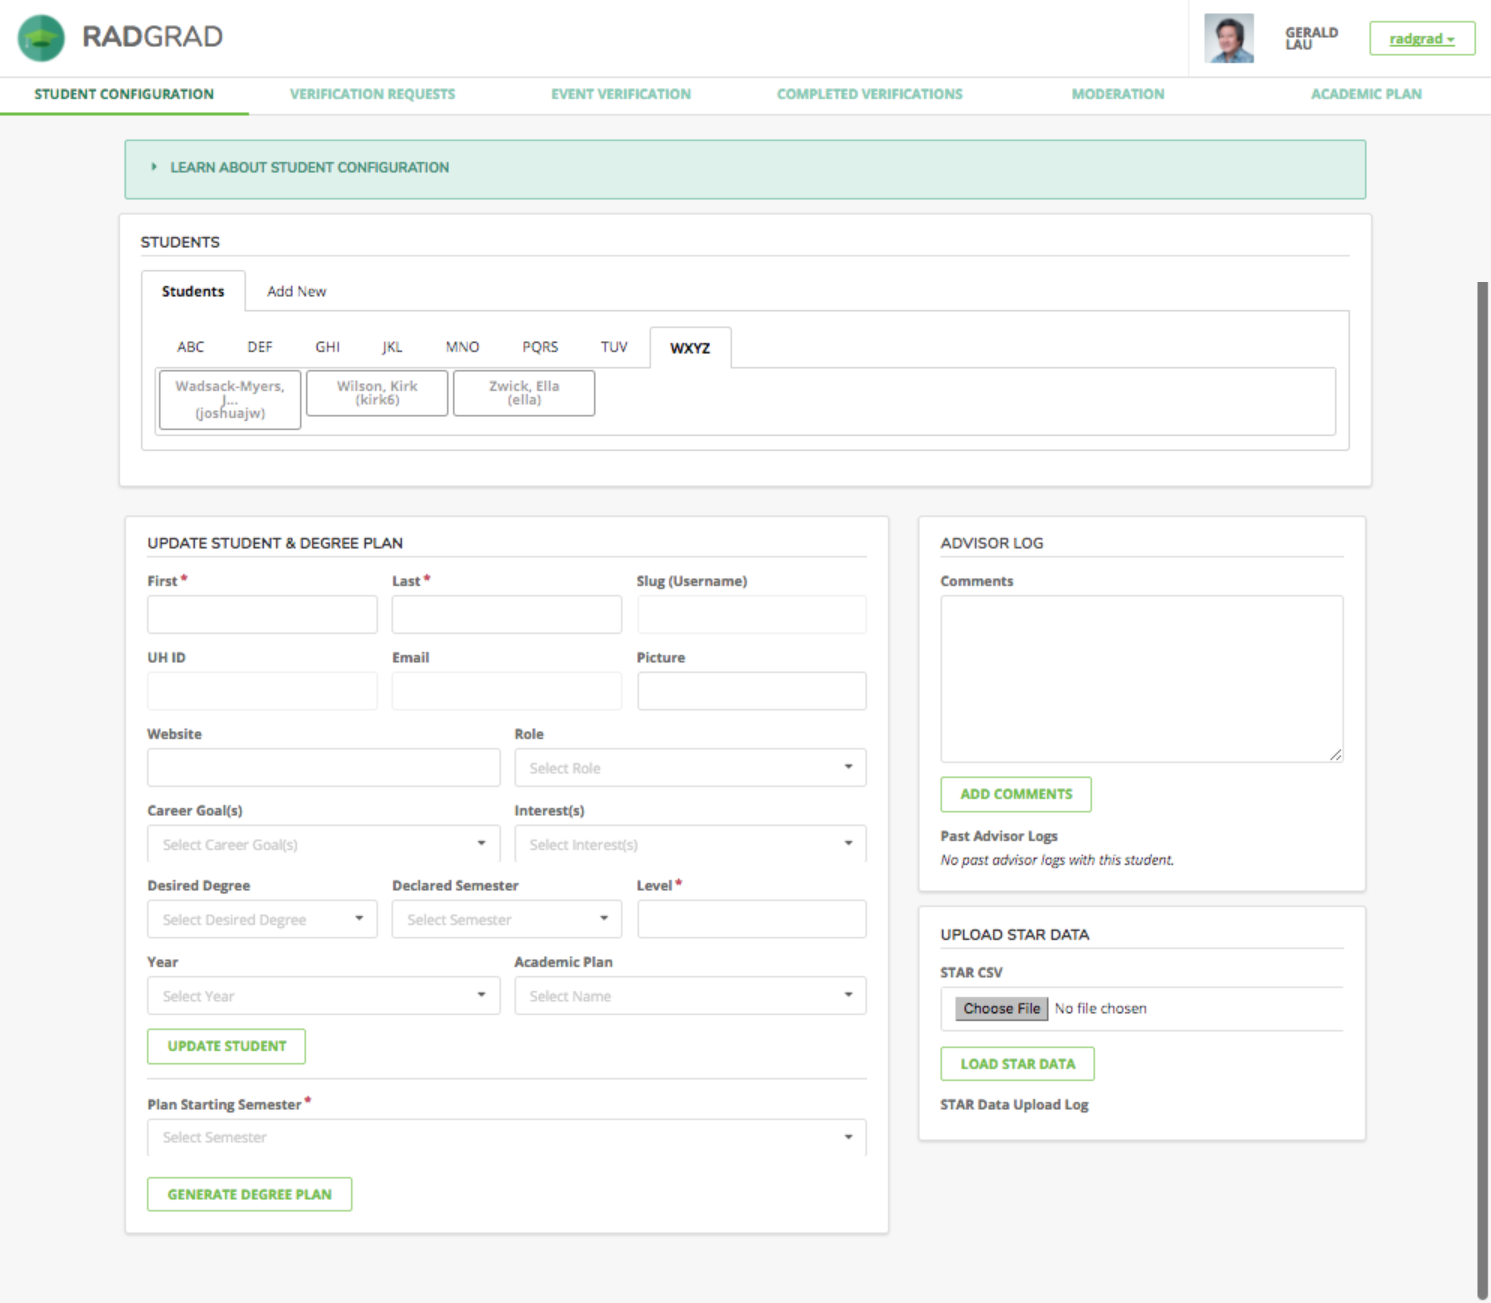
\includegraphics[width=1.0\textwidth]{advisor-student-configuration}
\caption{Advisor student configuration page.}
\label{advisor-student-configuration}
\end{figure}
On the student configuration page, advisors can add new students or update existing students (Figure ~\ref{advisor-student-configuration}). Existing students are listed alphabetically by last name. Advisors can update a student's first name, last name, picture, website, role, career goals, interests, desired degree, declared semester, level, year, academic plan, and plan starting semester from this interface. (Slug, email, and UH ID cannot be changed once the student has been added to RadGrad). On this page, advisors can also add advisor log comments and view any past advisor logs for a particular student. Advisors can also use this page to upload new star data and view past star data uploads. 
\subsection{Verification}
\begin{figure}[htbp!]
\centering
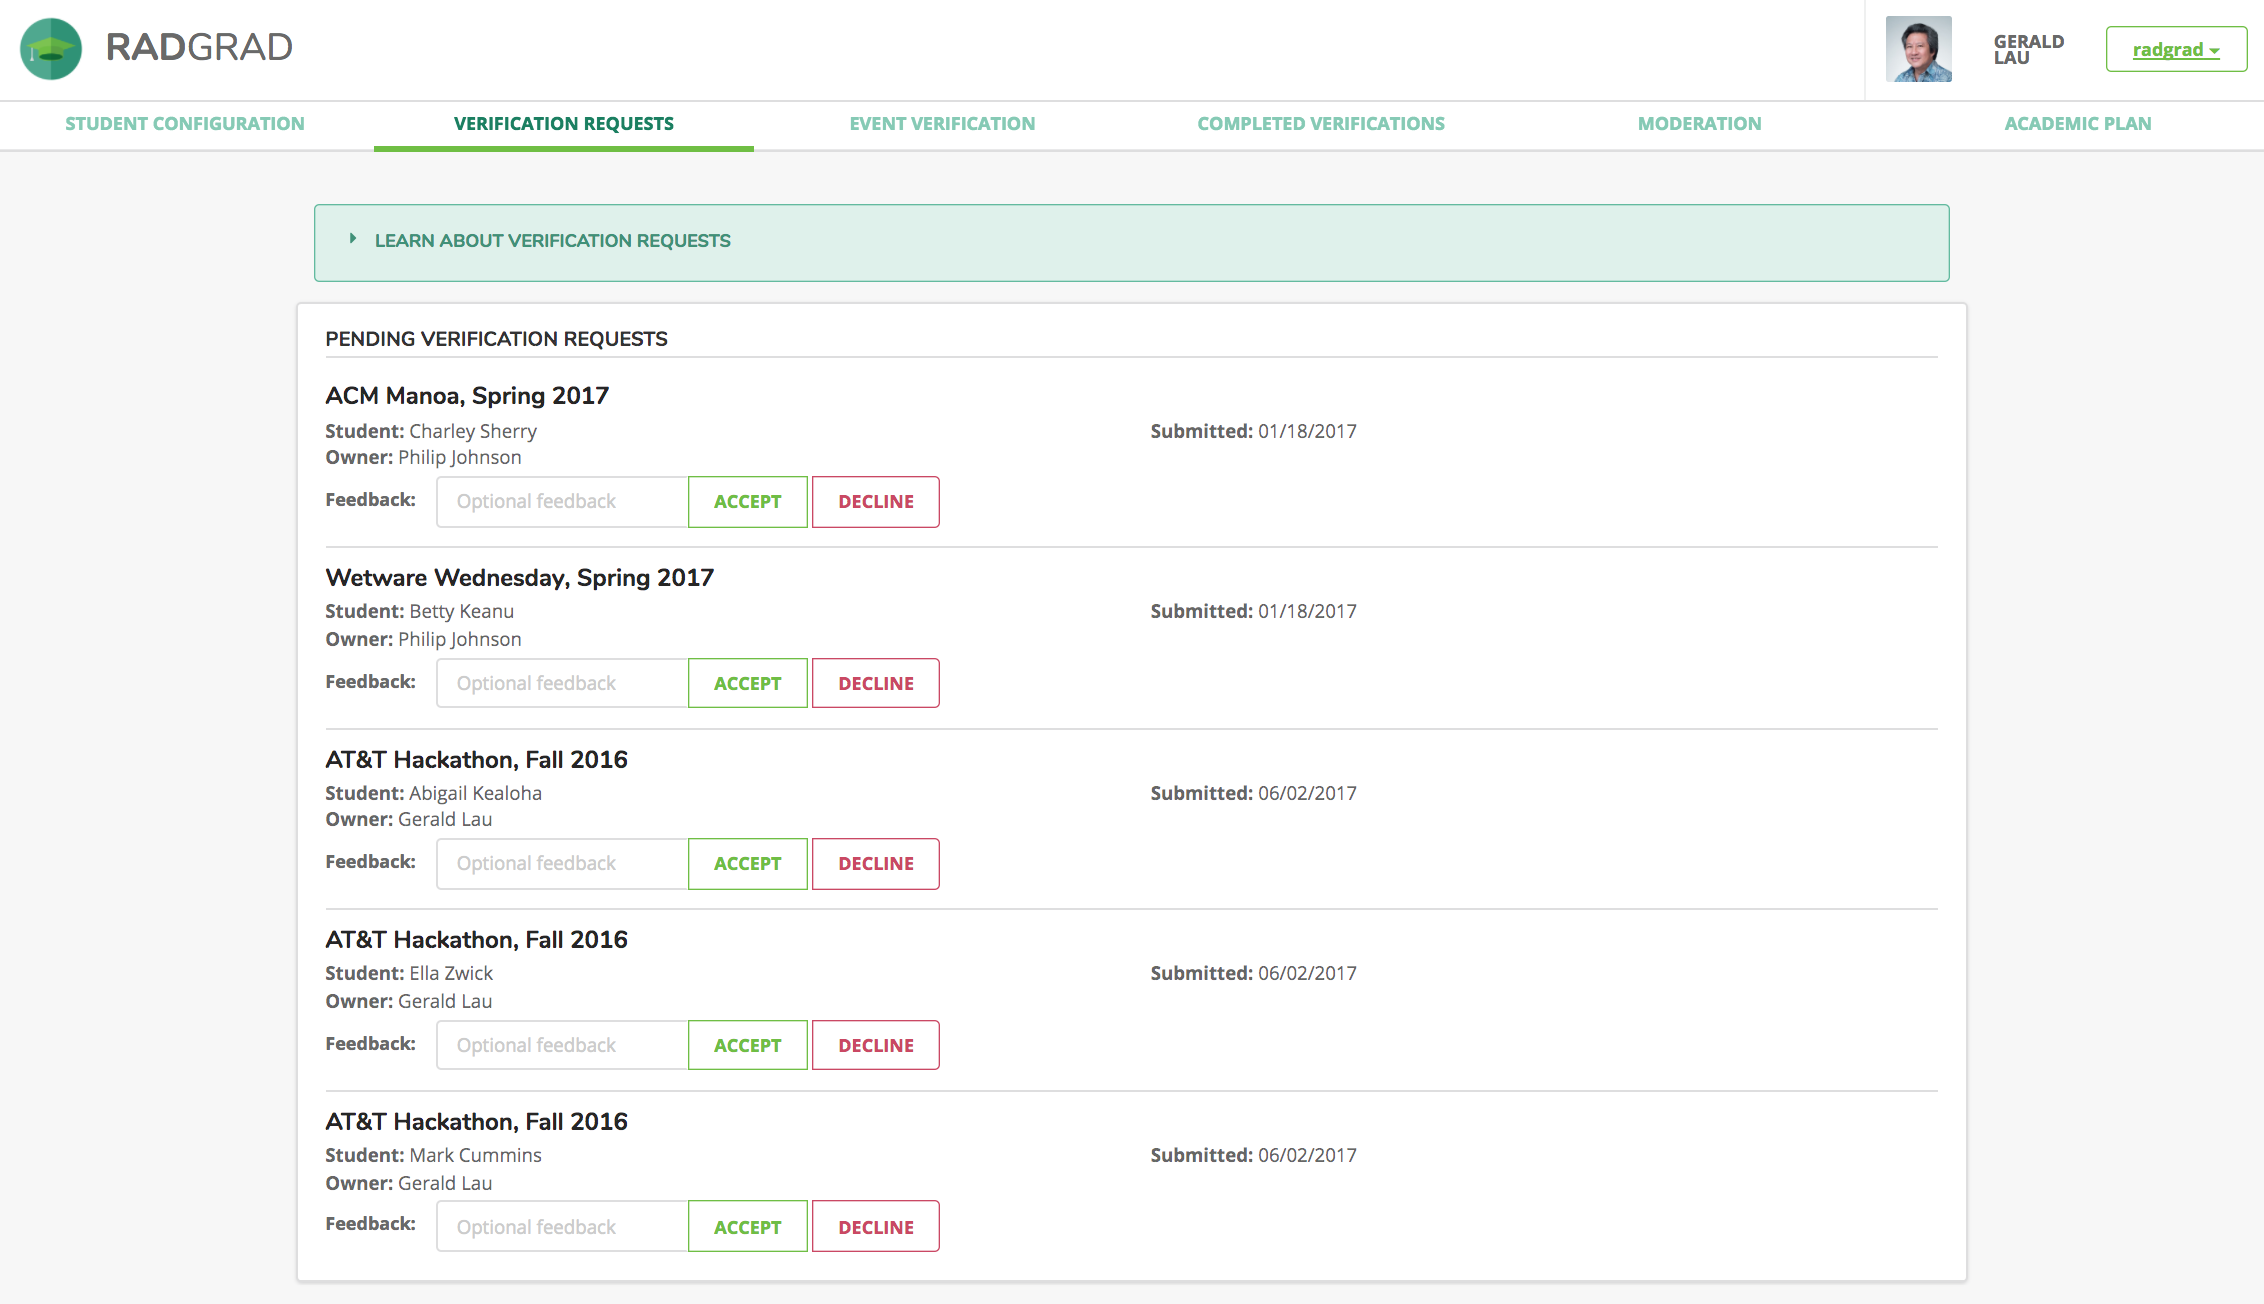
\includegraphics[width=1.0\textwidth]{advisor-verifications}
\caption{Advisor pending verifications page.}
\label{advisor-verifications}
\end{figure}

\begin{figure}[htbp!]
\centering
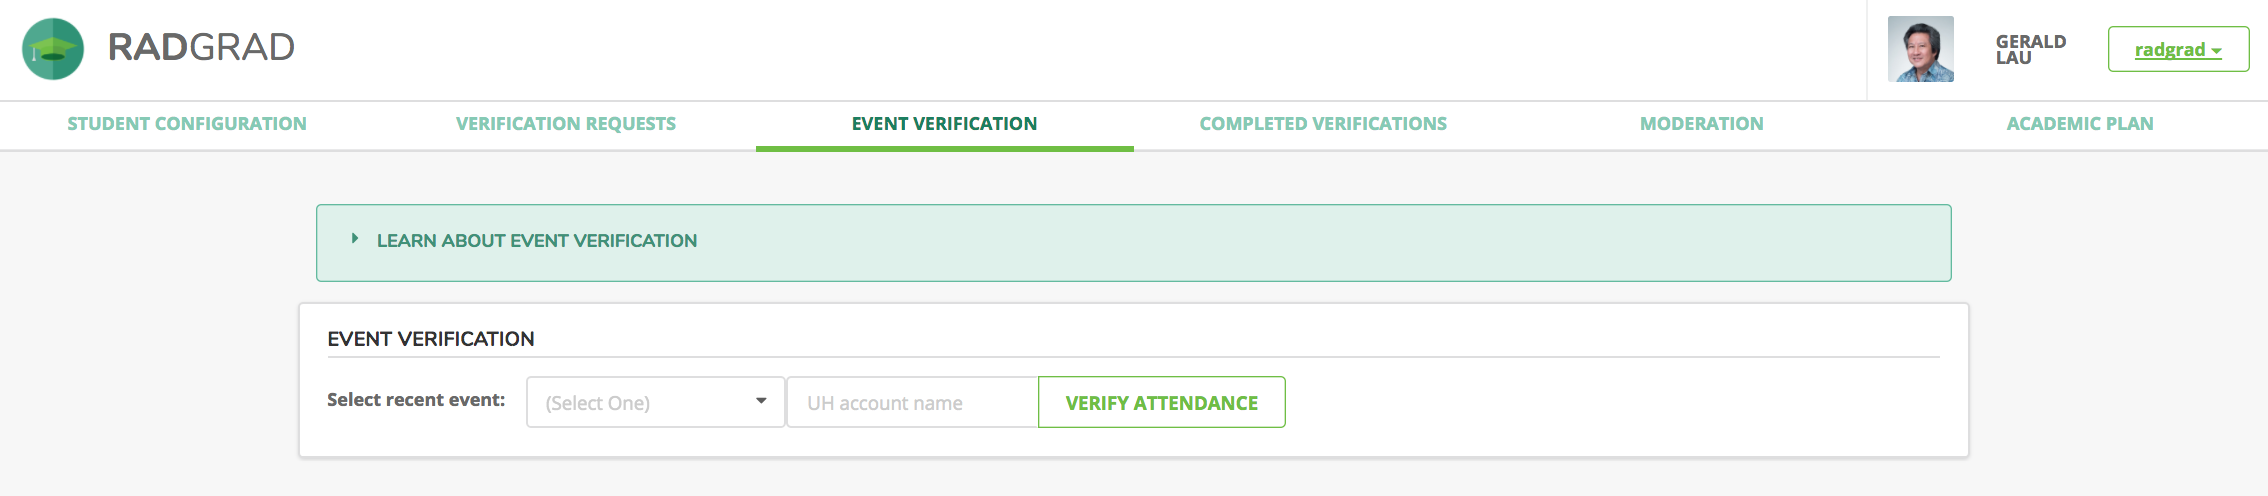
\includegraphics[width=1.0\textwidth]{advisor-eventverification}
\caption{Advisor event verifications page.}
\label{advisor-event-verifications}
\end{figure}

\begin{figure}[htbp!]
\centering
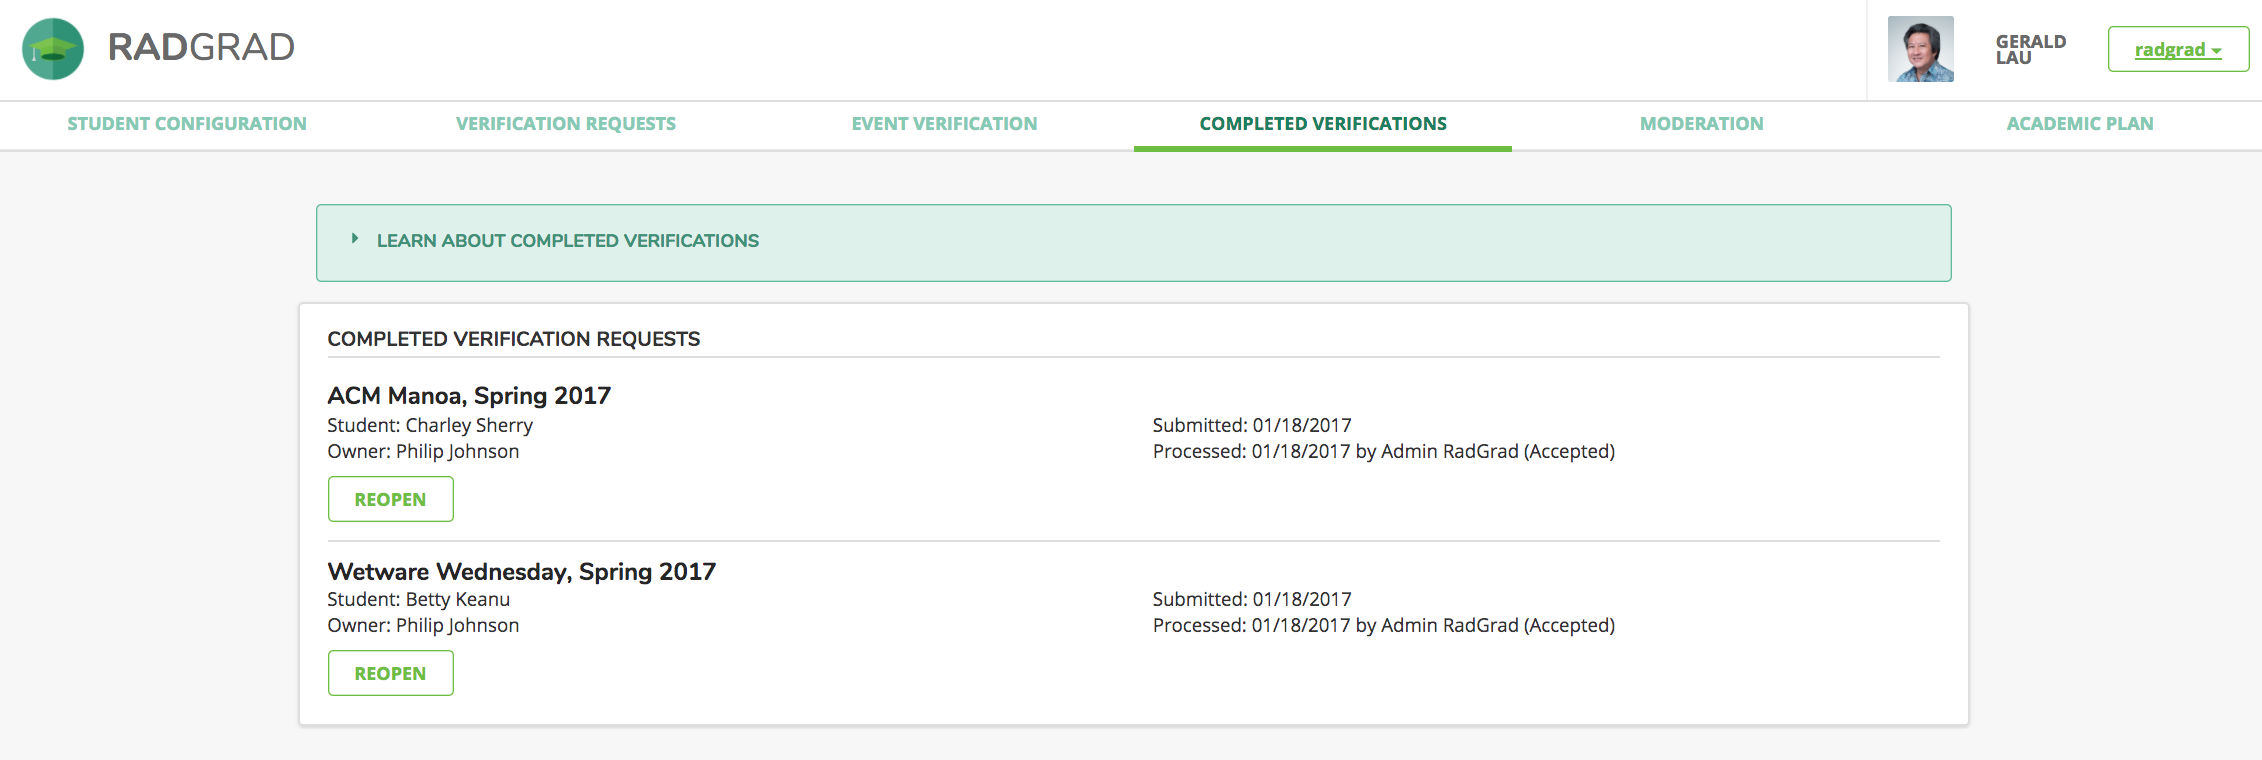
\includegraphics[width=1.0\textwidth]{advisor-completedverifications}
\caption{Advisor completed verifications page.}
\label{advisor-completed-verifications}
\end{figure}
Advisors can verify a student's completion of an opportunity in two ways: with a pending verification (Figure ~\ref{advisor-verifications}), and with an event verification (Figure ~\ref{advisor-event-verifications}). If an advisor is physically at an event, and needs to quickly verify a large amount of students, he can use the event verification. In this interface, the advisor simply chooses the event from a dropdown selection of recent events, and then types in the student's UH account name and clicks ``Verify Attendance." If an advisor is not physically present, a student can send a verification request through RadGrad. These requests show up as pending verifications. Advisors can choose to accept or decline these verifications. If they decide to decline, they can leave feedback for the student, and the student can resubmit as many times as they choose. Adivsors can view completed verifications (Figure ~\ref{advisor-completed-verifications}) to either simply check past verifications or to reopen a verification.
\subsection{Moderation}
\begin{figure}[htbp!]
\centering
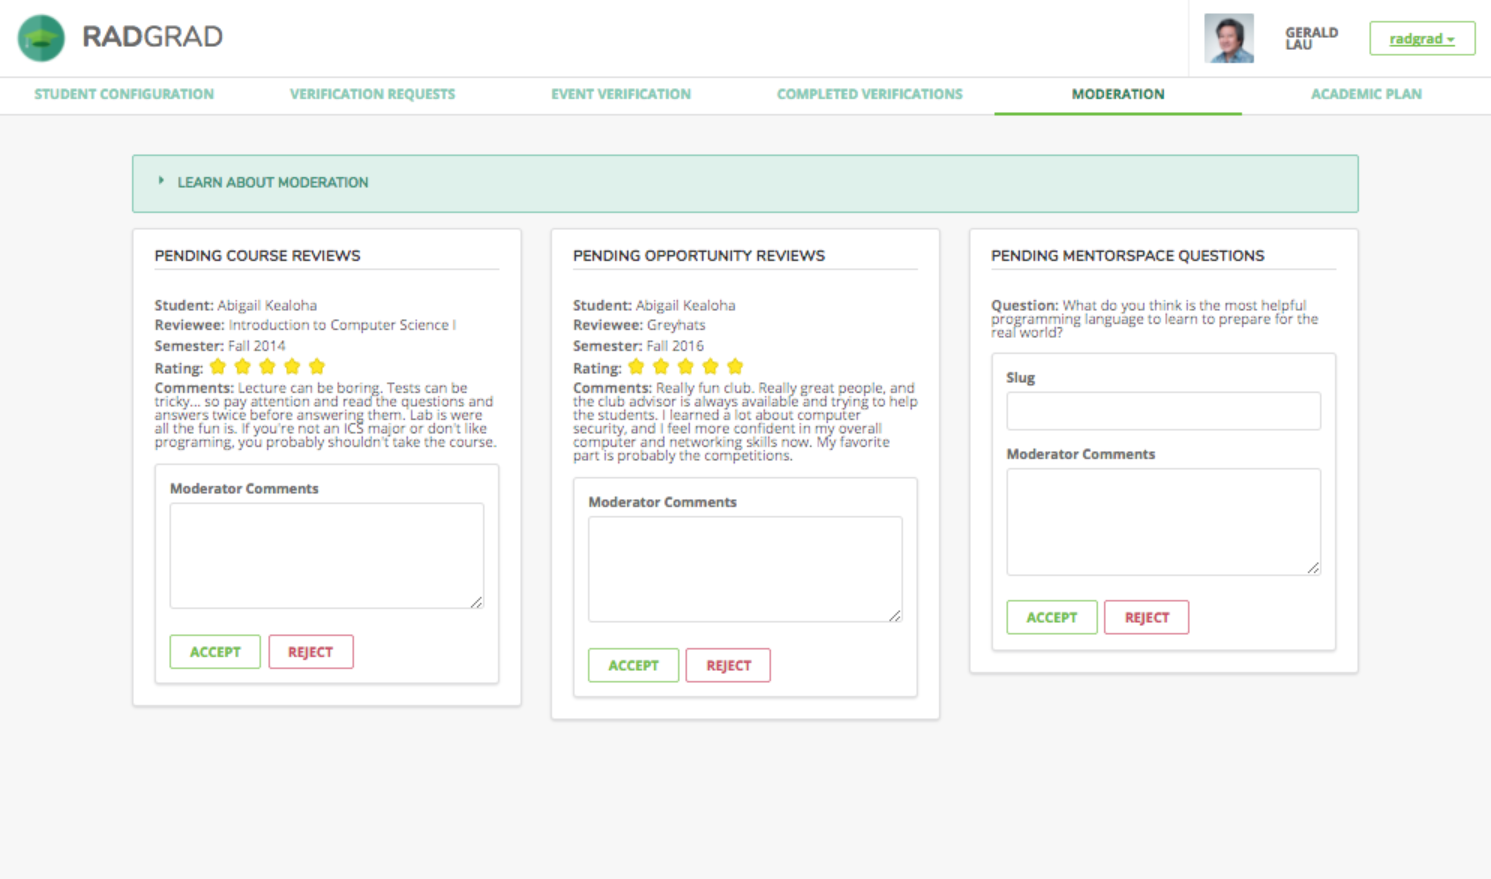
\includegraphics[width=1.0\textwidth]{advisor-moderation}
\caption{Advisor moderation page.}
\label{moderation}
\end{figure}
Advisors can use the moderation page to moderate course reviews, opportunity reviews, and MentorSpace questions (Figure ~\ref{moderation}). Advisors can choose to either accept or deny these posts. In the case of denial, advisors can leave reasons for denial so that the student can edit and resubmit their post accordingly. 
\subsection{Academic Plan}
\begin{figure}[htbp!]
\centering
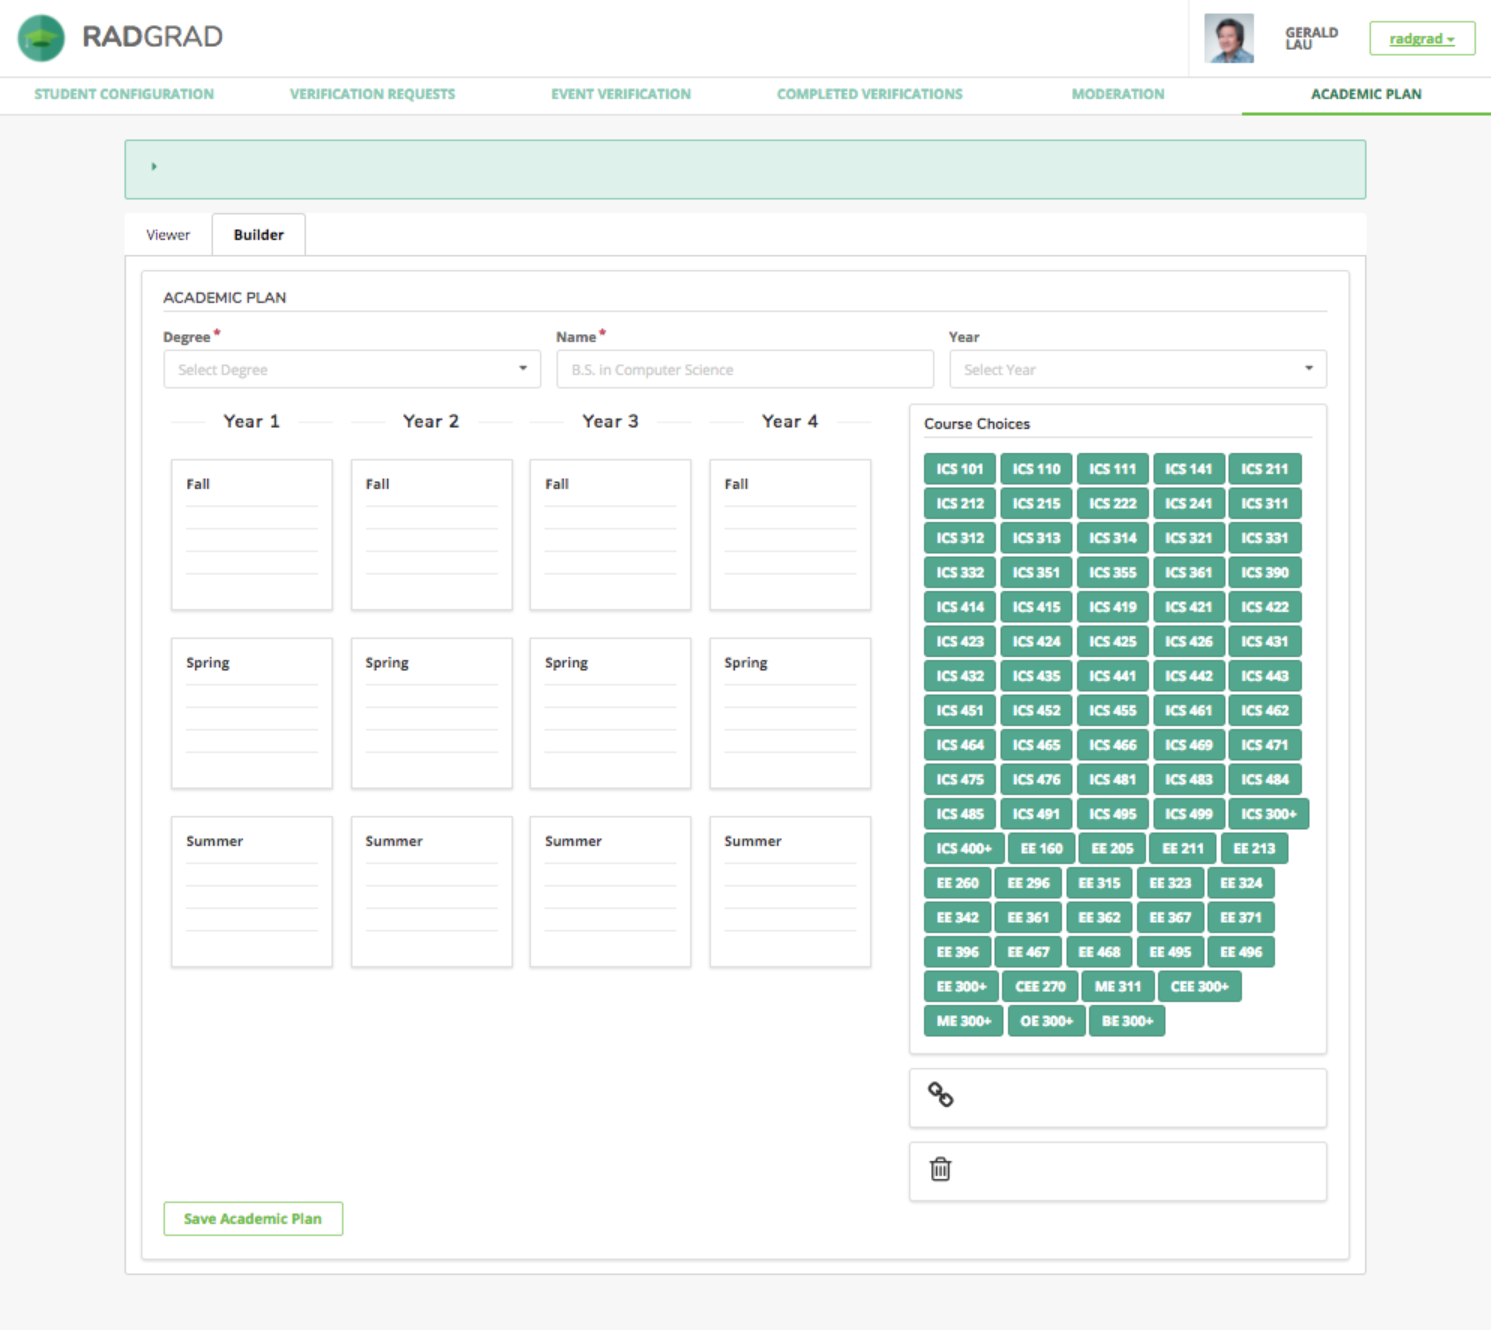
\includegraphics[width=1.0\textwidth]{advisor-academic-plan}
\caption{Advisor academic plan page.}
\label{academic-plan}
\end{figure}
The academic plan page is the only place on RadGrad that allows the user to build academic plans (Figure ~\ref{academic-plan}). There are two tabs: Viewer and Builder. The viewer allows the advisor to choose a year and a plan name, and view the four year plan for that plan. To make any edits to an existing plan or add a new plan, advisors can go over to the builder, which allows them to name a new academic plan with a degree, name, and year. The advisor can then build the four year plan easily by dragging and dropping possible courses onto the initially empty plan. Some plans have more complex requirements than a single courses (i.e. a student must take one course from one of the four groups: ICS312 or ICS331, ICS 313 or ICS361, ICS351 or ICS451, or ICS355). For requirements like this, advisors can easily create groupings by dragging courses to the box with the link icon. Once a complex requirement is completely built, it can be dragged directly onto the plan. If an advisor no longer needs a certain requirement, they can delete it by dragging it to the trash can icon. 

\section{Faculty Mode}
\subsection{Profile}
\begin{figure}[htbp!]
\centering
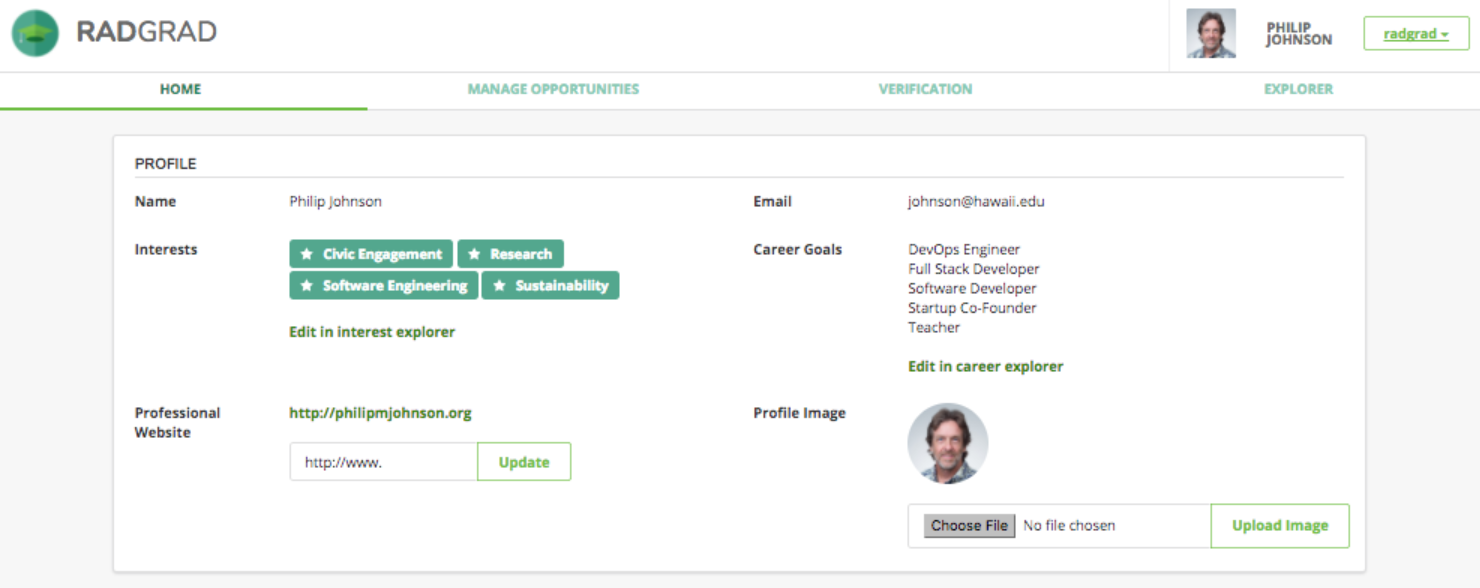
\includegraphics[width=1.0\textwidth]{faculty-profile}
\caption{Faculty profile page.}
\label{faculty}
\end{figure}
Faculty can use the profile page to view and edit their profile, which reflects how others will see them on RadGrad (Figure ~\ref{faculty}). On this page, faculty can update their photo and information about their website. Faculty can personalize their profiles in a way that accurately communicates their background and research to students. 
\subsection{Manage Opportunities}
\begin{figure}[htbp!]
\centering
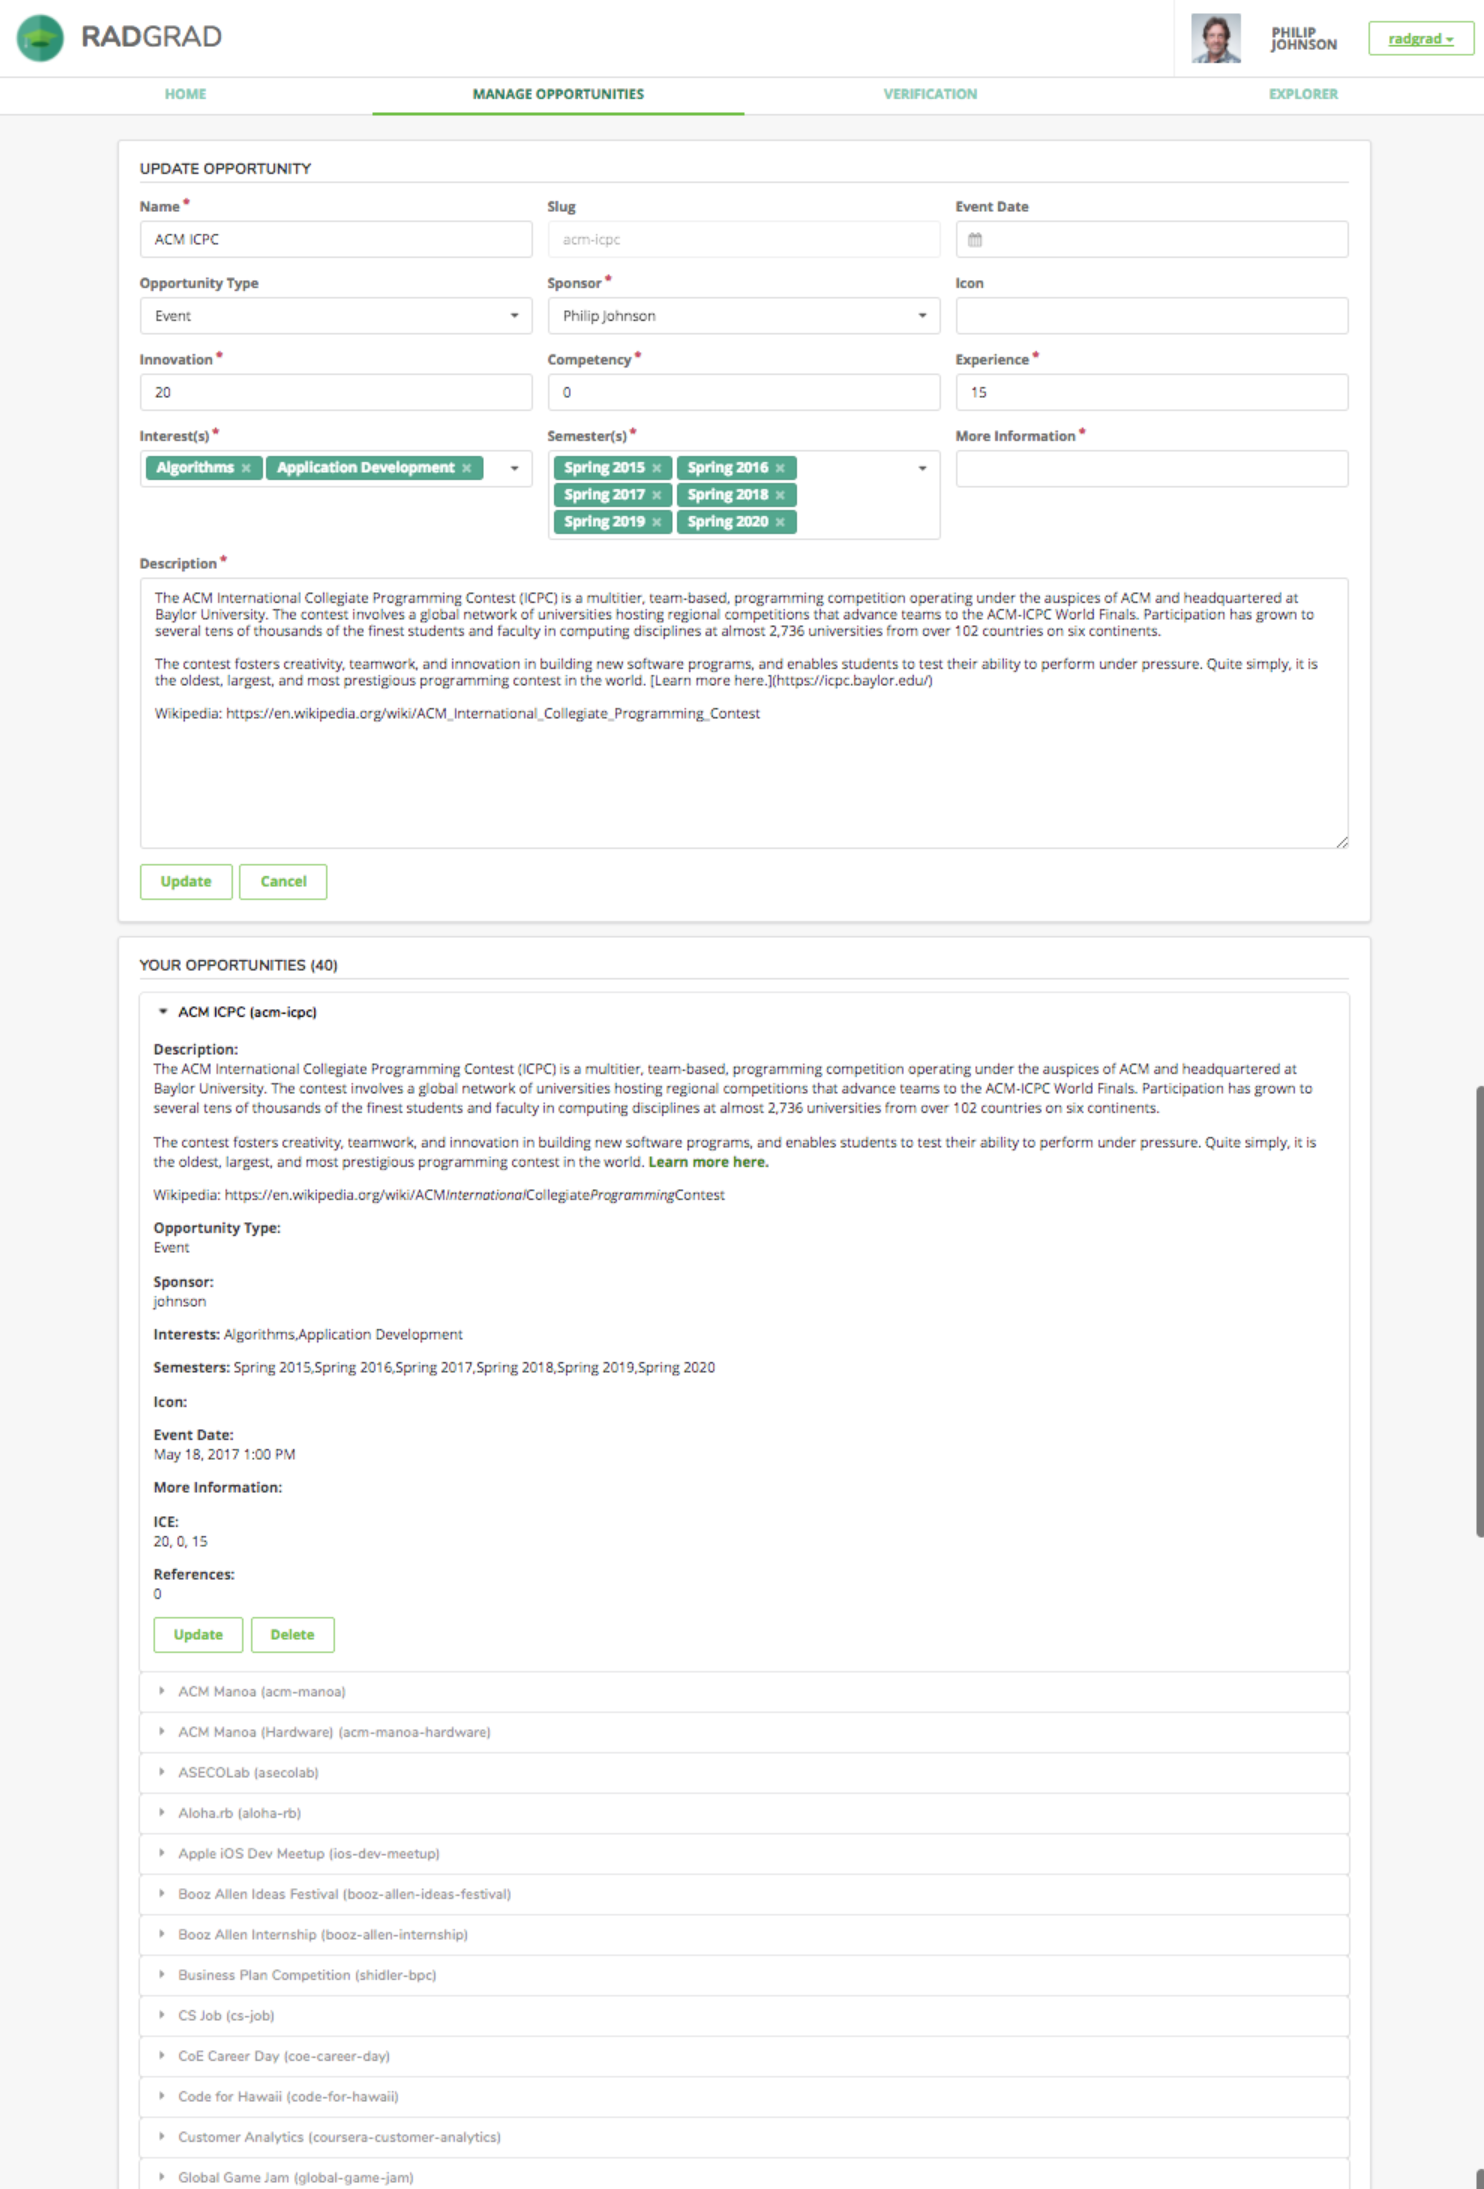
\includegraphics[width=1.0\textwidth]{faculty-opportunity}
\caption{Faculty Manage Opportunities page.}
\label{faculty-manage-opportunities}
\end{figure}
Faculty can use the manage opportunities page to easily view, add, edit, or delete their sponsored opportunities (Figure ~\ref{faculty-manage-opportunities}). They can also view other opportunities, but they can only edit their own. Faculty can edit their opportunities at any time.
\subsection{Verification}
Faculty have the same verification interface as advisors, except they can only view their own verifications for their own sponsored opportunities. 
\subsection{Explorers}
Faculty view the same explorer as students, except they cannot add courses or opportunities, and they cannot leave any type of review. However, they can use the explorer to add interests and career goals. Also, the opportunity explorer conveniently shows the faculty's sponsored opportunities at the top of their opportunity list for quick access.

\section{Mentor Mode}
\subsubsection{Profile}
\begin{figure}[htbp!]
\centering
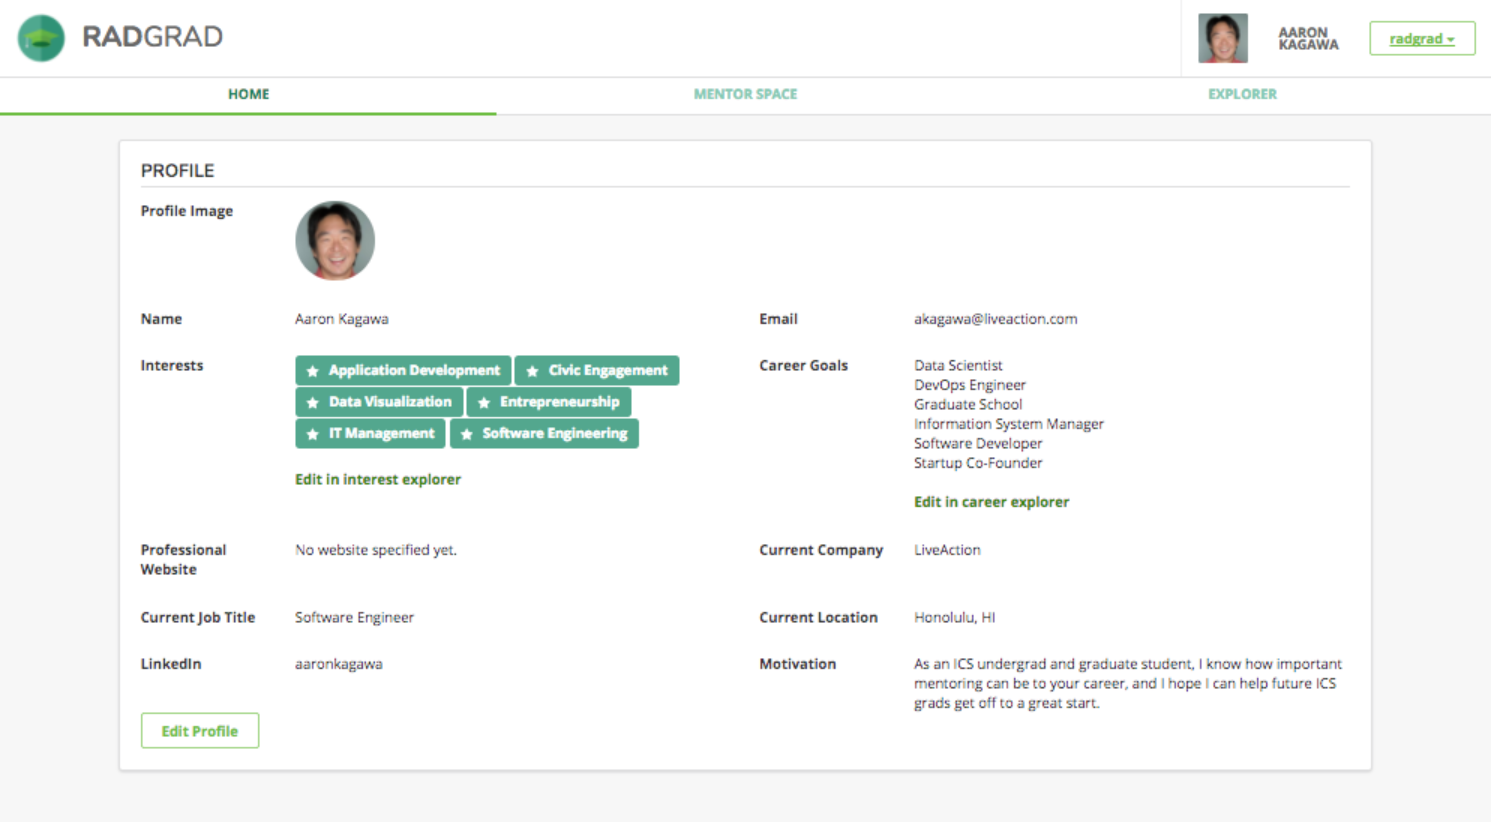
\includegraphics[width=1.0\textwidth]{mentor-profile}
\caption{Mentor profile page.}
\label{mentor-profile}
\end{figure}
Mentors can use the profile page to view and edit their profile, which reflects how others will see them on RadGrad (Figure ~\ref{mentor-profile}). On this page, mentors can update their photo and information about their website, company, job title, location, LinkedIn, and motivation for becoming a mentor. Mentors can personalize their profiles in a way that accurately communicates their background and willingness to help to the students. 
\subsubsection{MentorSpace}
\begin{figure}[htbp!]
\centering
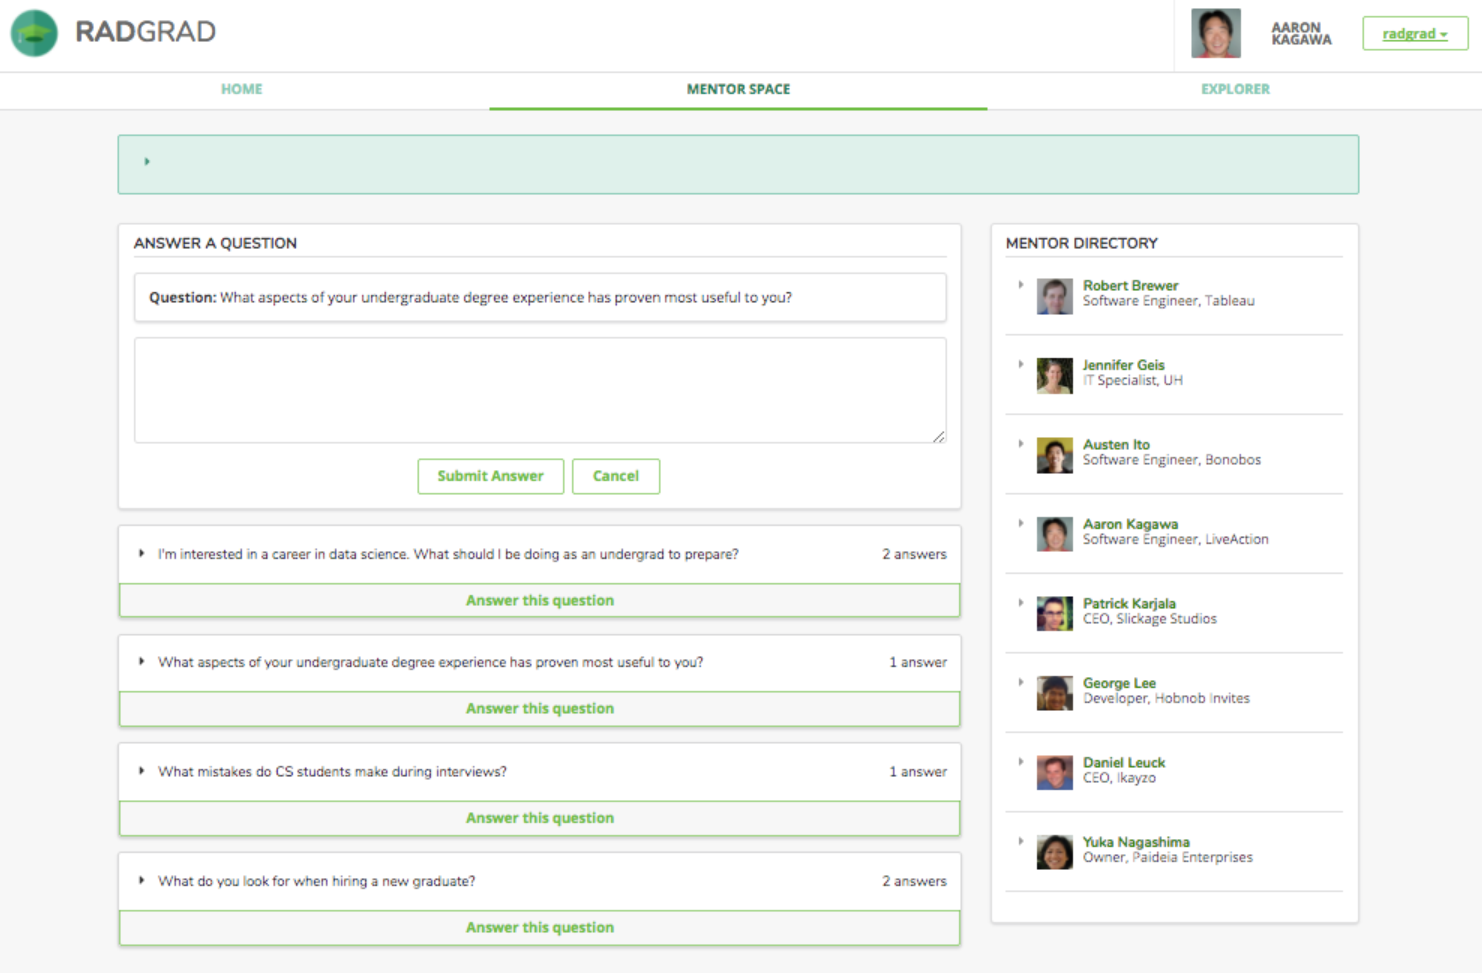
\includegraphics[width=1.0\textwidth]{mentor-mentorspace}
\caption{Mentor MentorSpace Page.}
\label{mentor-mentorspace}
\end{figure}
Mentors view the same MentorSpace that students do, except each question has an ``Answer this question" or ``Edit your answer" button (Figure ~\ref{mentor-mentorspace}). Clicking on this button brings up a form at the top of the page, which mentors can use to either submit a new answer or revise their existing answer. 
\subsubsection{Explorer}
Mentors view the same explorer as students, except they cannot add courses or opportunities, and they cannot leave any type of review. However, they can use the explorer to add interests and career goals.

\section{Administrator Mode}
\subsection{Retrieve User}
\begin{figure}[htbp!]
\centering
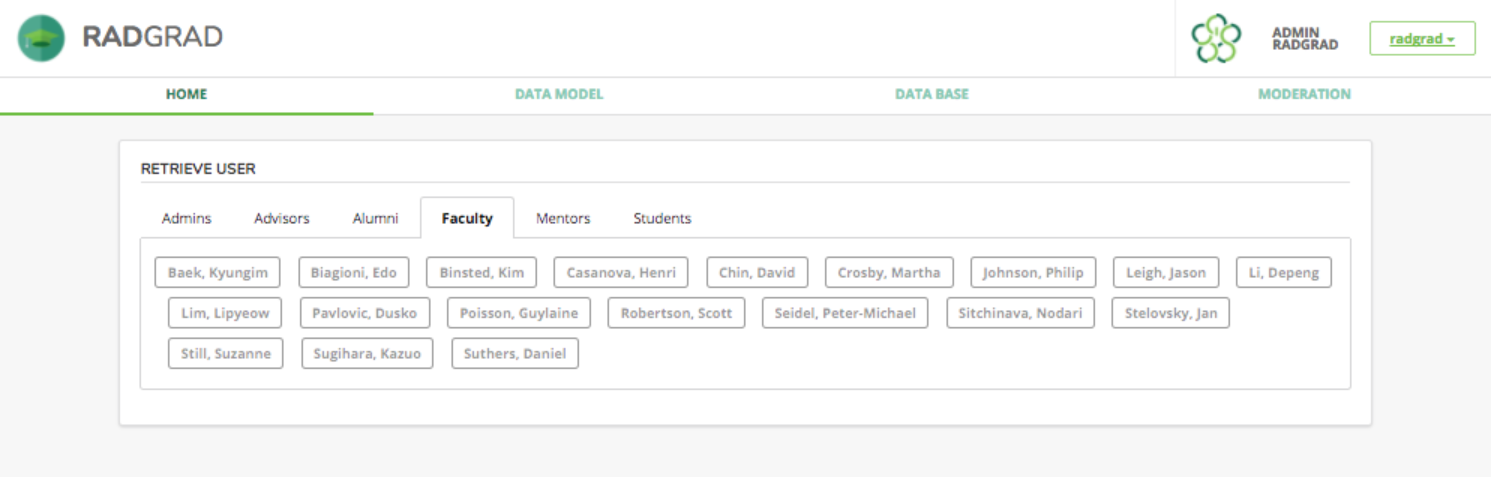
\includegraphics[width=1.0\textwidth]{admin-retrieve-user}
\caption{Administrator Retrieve User page.}
\label{admin-retrieve-user}
\end{figure}
On the Administrator home page, an administrator can access any user's account (Figure ~\ref{admin-retrieve-user}). Users are organized by role (on tabs) and then alphabetically by last name. Clicking on the user's name will lead to their profile. Administrators can use this for testing or troubleshooting purposes. On the student tab, there is also a button to update student levels. Clicking this button will automatically recalculate and set the levels for all of the students.

\subsection{Data Model}
\begin{figure}[htbp!]
\centering
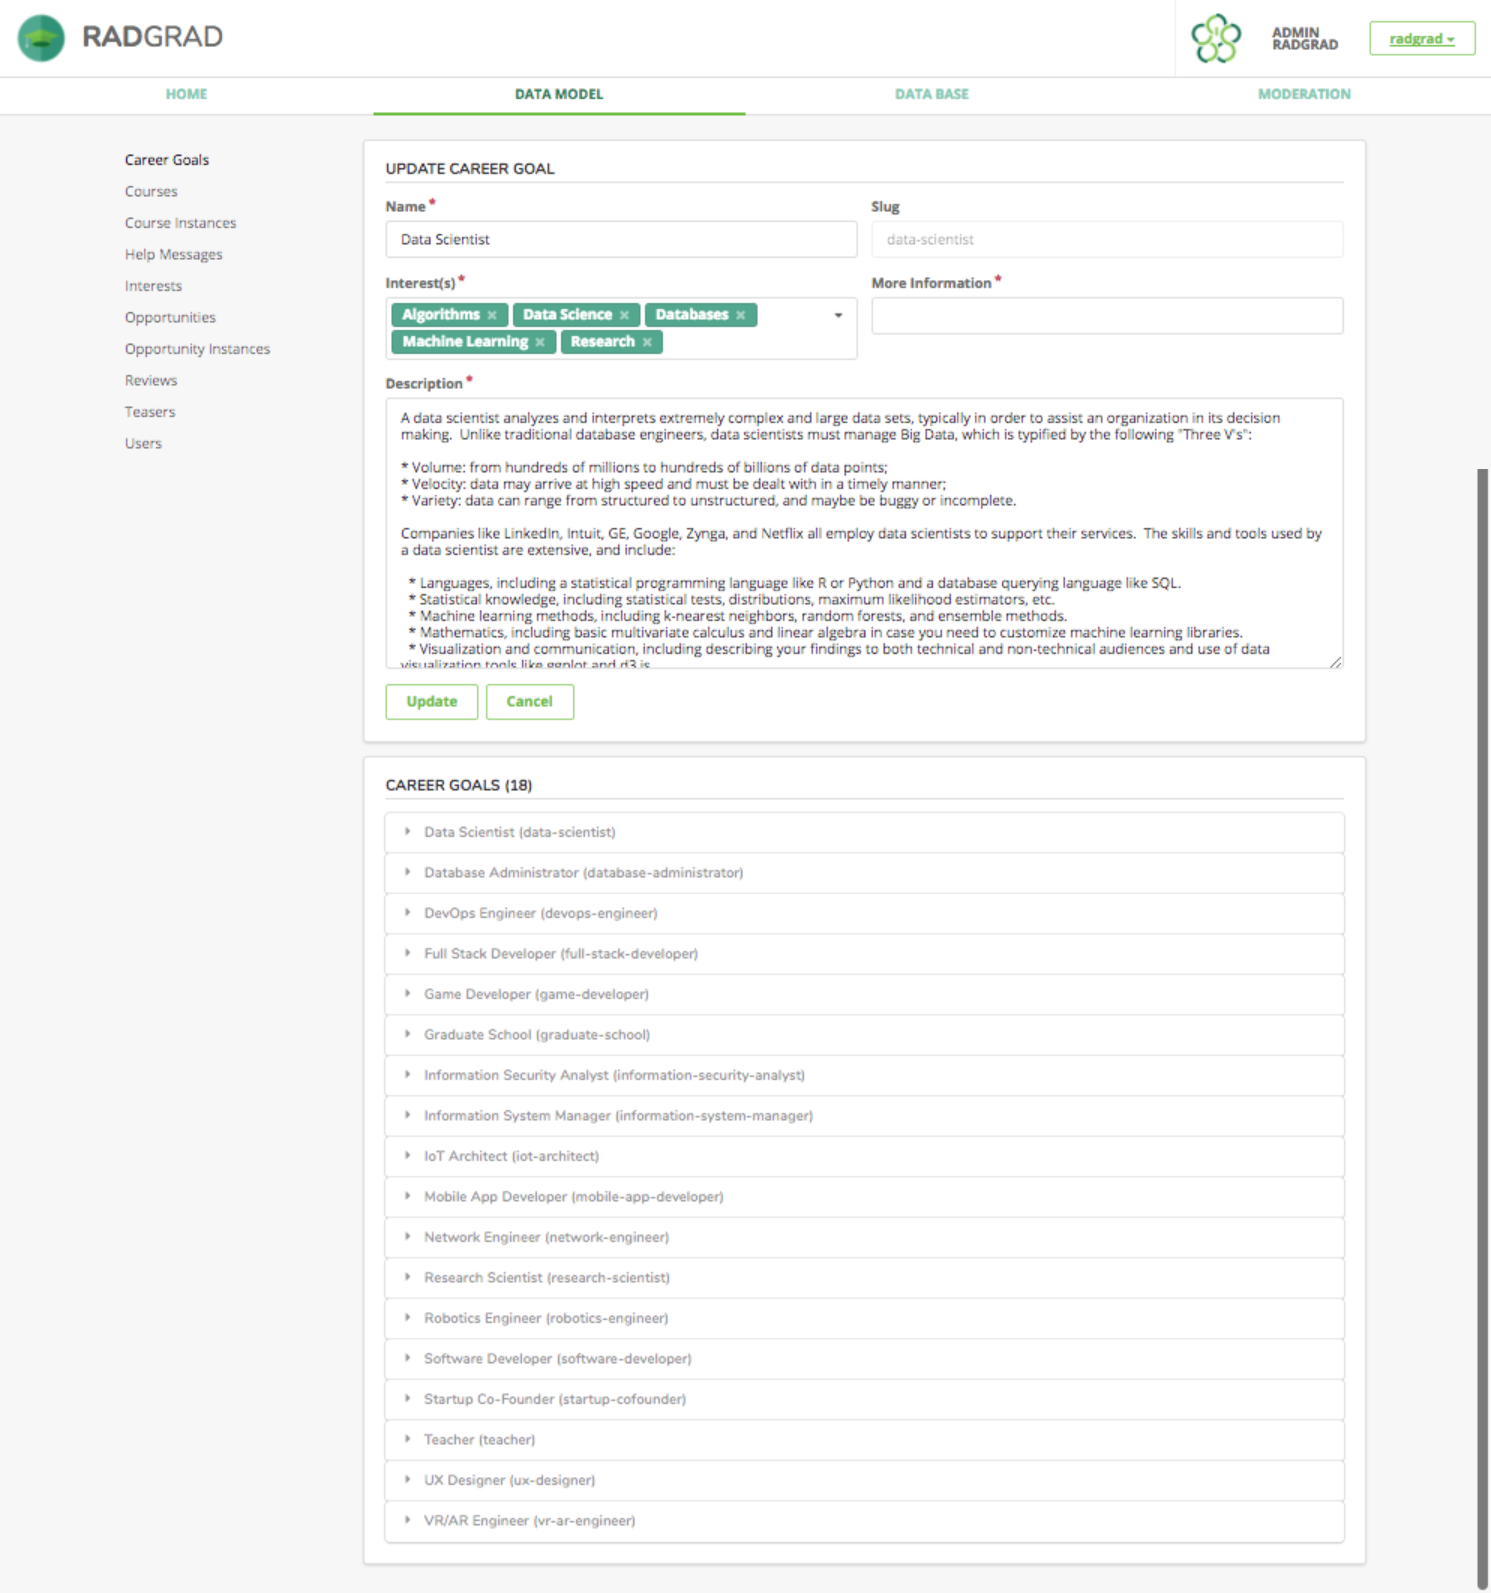
\includegraphics[width=1.0\textwidth]{admin-datamodel}
\caption{Administrator Data Model page.}
\label{admin-datamodel}
\end{figure}
The data model page allows administrators to view, add, edit, and delete items from the data model (Figure ~\ref{admin-datamodel}). The menu on the left lists all collections. When an administrator clicks on a collection, they will see a form, which they can use manipulate items in that collection. Below the form, they can view a list of all existing collection items. 
\subsection{Data Base}
\begin{figure}[htbp!]
\centering
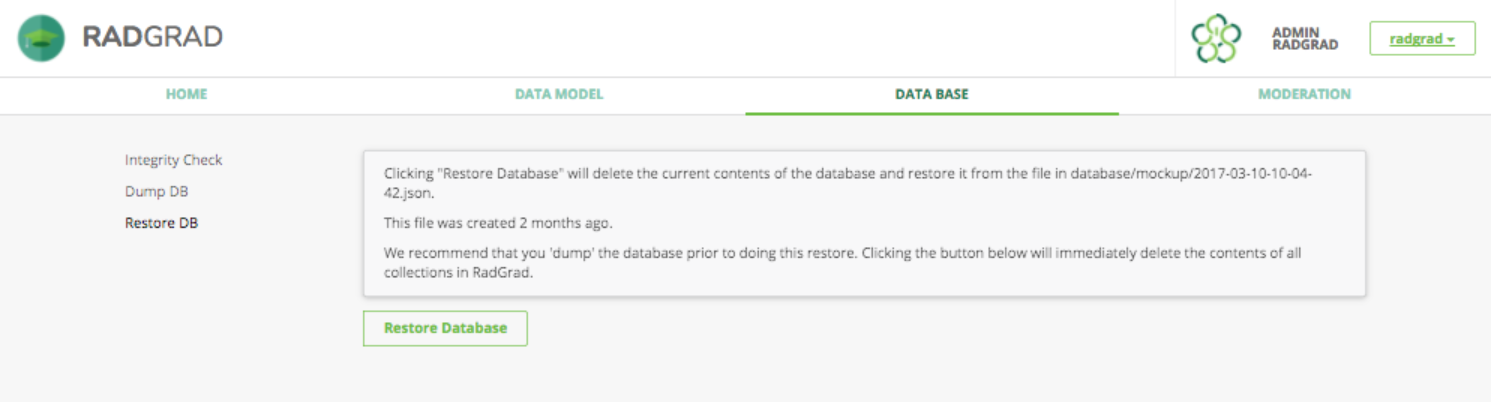
\includegraphics[width=1.0\textwidth]{admin-database}
\caption{Administrator Data Base page.}
\label{admin-database}
\end{figure}
The database page allows administrators to easily run an integrity check on the database, dump the database, and restore the database (Figure ~\ref{admin-database}). The integrity check tests every item in the database to make sure that all parts of it are valid. Dumping the database saves the current state of the database to a JSON file and downloads it to your computer. Restoring the database deletes the current database and reloads an earlier version from a JSON file. Administrators can use this in backup and testing situations.
\subsection{Moderation}
Administrators have the same moderation page as advisors. 